% LaTeX source for ``การเรียนรู้ของเครื่องสำหรับเคมีควอนตัม (Machine Learning for Quantum Chemistry)''
% Copyright (c) 2022 รังสิมันต์ เกษแก้ว (Rangsiman Ketkaew).

% License: Creative Commons Attribution-NonCommercial-NoDerivatives 4.0 International (CC BY-NC-ND 4.0)
% https://creativecommons.org/licenses/by-nc-nd/4.0/

\chapter{การเรียนรู้เชิงลึก}
\label{ch:deep_learning}

ในบทนี้ผู้อ่านจะได้ศึกษาการเรียนรู้เชิงลึกหรือ Deep Learning ซึ่งเป็นหนึ่งใน Buzzword\footnote{สิ่งที่กำลังเป็นที่พูดถึงหรือได้รับความนิยม
    โดยที่ฟังแล้วก็อาจจะเป็นคำเก๋ ๆ} ที่หลาย ๆ คนต่างก็พูดถึงในช่วงระยะเวลา 10 ปีที่ผ่านมาโดยเฉพาะในช่วงเวลาที่ผู้เขียนกำลังเขียนหนังสือเล่มนี้
ไม่ว่าจะเป็นวงการหรืออาชีพไหน ๆ ต่างก็มีการนำ Deep Learning เข้าไปประยุกต์ใช้ทั้งนั้นและแน่นอนว่าหนึ่งในนั้นก็คือการนำมาประยุกต์ใช้%
ในงานวิจัยทางด้านเคมี เนื่องจากว่าข้อมูลที่นักเคมีมีอยู่ในมือนั้นมากมายมหาศาล ไม่ว่าจะเป็นข้อมูลเกี่ยวกับสภาวะของปฏิกิริยาเคมี (อุณหภูมิและ%
ความดันที่ใช้ เป็นต้น), ตัวเร่งปฏิกิริยาที่มีประสิทธิภาพสูงสำหรับปฏิกิริยาแต่ละประเภท, และหมู่ฟังก์ชันนอลที่นำมาใช้ในการสังเคราะห์โมเลกุลยา
ดังนั้นจึงน่าสนใจว่า Deep Learning จะช่วยนักเคมีในการขับเคลื่อนงานวิจัยได้อย่างไรและมากน้อยแค่ไหน

ถ้าจะให้นิยาม Deep Learning แบบเข้าใจง่าย ๆ โดยใช้การยกตัวอย่างก็คือเป็นเทคนิคในการสร้างโมเดลคอมพิวเตอร์ที่ได้จากการฝึกฝนให้สามารถ%
ทำงานได้เหมือนมนุษย์แบบที่มีสภาวะในการทำงานที่ซับซ้อนมาก ๆ (ที่มาของคำว่าลึกหรือ Deep) เช่น การสังเกต การจดจำคำพูด การระบุภาพ
หรือการคาดการณ์ แทนที่จะจัดระเบียบข้อมูลที่จะคำนวณผ่านทางสมการที่กำหนดไว้ล่วงหน้า Deep Learning จะกำหนดค่าพารามิเตอร์พื้นฐาน%
เริ่มต้นเกี่ยวกับข้อมูล (Hyperparameters) และฝึกให้คอมพิวเตอร์เรียนรู้ด้วยตัวเองโดยการจดจำรูปแบบโดยการใช้การประมวลผลหลายชั้น
อีกหนึ่งวัตถุประสงค์ของการพัฒนา Deep Learning นั้นก็คือการสร้าง Neural Network ที่สามารถสกัดหรือดึงสิ่งที่ซ่อนอยู่ภายในข้อมูล (Hidden
Features) ออกมาได้ด้วยตัวของโมเดลเองโดยปราศจากการช่วยเหลือจากผู้ใช้งานหรือมนุษย์

\begin{figure}[H]
    \centering
    \includegraphics[width=0.7\linewidth]{fig/wisard.png}
    \caption{เครื่องการเรียนรู้เชิงลึก WISARD เครื่องแรกของโลก ณ พิพิธภัณฑ์วิทยาศาสตร์ กรุงลอนดอน ประเทศอังกฤษ
        (เครดิตภาพ: รังสิมันต์ เกษแก้ว)}
    \label{fig:wisard}
\end{figure}

จริง ๆ แล้ว Deep Learning นั้นถือว่าเป็นอัลกอริทึมประเภทหนึ่งของ Neural Network ซึ่งเป็นเทคนิคปัญญาประดิษฐ์แบบหนึ่งที่ถูกพัฒนาขึ้นมา%
เพื่อศึกษารูปแบบที่แน่นอนของข้อมูลเรียกว่า \textit{การรับรู้รูปแบบ (Pattern Recognition)} ซึ่งเป็นกระบวนที่ทำงานเลียนแบบ (Mimic)
สมองของมนุษย์ในการแยกแยะความจำเพาะเจาะจงบางอย่างออกมาจากข้อมูลที่ป้อนเข้าไป ภาพที่ \ref{fig:wisard} แสดงเครื่อง WISARD
ซึ่งเป็นคอมพิวเตอร์เครื่องแรกของโลกที่ถูกสร้างขึ้นมาในปี ค.ศ. 1981 สำหรับการคำนวณ Deep Learning

ผู้เขียนขอสรุปสั้น ๆ เพื่อไม่ให้สับสนดังนี้ \textit{\enquote{Deep Learning ทุกรูปแบบเป็น Machine Learning แต่ว่าไม่ใช่ Machine
        Learning ทุกเทคนิคที่จะเป็น Deep Learning}}

ในบทก่อนหน้านี้นั้นเราได้พูดถึง Supervised Learning กันไปแล้ว ซึ่งจะเป็นการทำนายค่า $y$ จากข้อมูลนำเข้า $x$ โดยเป็นการพิจารณาใน%
กรณีของการถดถอยเชิงเส้น ในลำดับถัดมา (ซึ่งก็คือในบทนี้) เราจะมาพิจารณากรณีที่พารามิเตอร์ของเรานั้นมีความไม่เป็นเชิงเส้น (Nonlinear)
กันครับ ซึ่งโมเดลปัญญาประดิษฐ์ที่ถูกนำมาใช้อย่างแพร่หลายนั้นก็คือ Neural Network นั่นเอง โดยเฉพาะ Deep Learning ที่ ณ ปัจจุบันได้มี%
การพัฒนาและปรับปรุงจนมีประสิทธิภาพที่สูงมาก ข้อดีอย่างหนึ่งของ Neural Network ก็คือสามารถจัดการกับข้อมูลที่มีความซับซ้อนที่มีจำนวน
Feature หลายร้อยหรือหลายพัน Feature ได้

%--------------------------
\section{การเรียนรู้ของโมเดลที่ไม่เป็นเชิงเส้น}
\label{sec:nonlinear_ml}
\idxboth{การเรียนรู้ของโมเดลที่ไม่เป็นเชิงเส้น}{Nonlinear Supervised Learning}
%--------------------------

สมมติว่าเรามี $\{(x^{(i)}, y^{(i)})\}^n_{i=1}$ ซึ่งเป็นตัวอย่างชุดข้อมูลฝึกสอน (Training Data) และเราจะเริ่มกันด้วยกรณีที่ง่ายที่สุด%
นั่นก็คือ $y^{(i)} \in \mathbb{R}$ และ $h_\theta(x) \in \mathbb{R}$

เราจะทำการกำหนด Loss Function หรือ Coss Function ขึ้นมาก่อน ซึ่งเราจะใช้ Least Square Cost Function สำหรับข้อมูลลำดับที่ $i$
นั่นก็คือคู่อันดับ $(x^{(i)} ,y^{(i)})$ ดังนี้

\begin{equation}\label{eq:loss}
    J^{(i)} (\theta) = \frac{1}{2} \left(h_\theta (x^{(i)}) - y^{(i)}\right)^2
\end{equation}

\noindent และกำหนด Mean-Square Cost Function สำหรับชุดข้อมูลดังนี้

\begin{equation}\label{eq:mse_loss}
    J(\theta) = \frac 1 n \sum_{i=1}^n J^{(i)}(\theta)
\end{equation}

\noindent ซึ่งผู้อ่านอาจจะสังเกตได้ว่าสมการข้างต้นนั้นจะเหมือนกับในกรณีของ Linear Regression เว้นแต่จะต่างกันตรงที่เราได้มีการเพิ่ม $1/n$
เข้าไปในด้านหน้าของ Cost Function ซึ่งเป็นการคูณ Cost Function ด้วยปริมาณสเกลาร์นั่นเอง โดยการคูณแบบนี้จะไม่ทำให้จุดต่ำสุดสัมพัทธ์
(Local minima) และจุดต่ำสุดสัมบูรณ์ (Global Minima) เปลี่ยนไป นอกจากนี้ผู้อ่านจะต้องทำความเข้าใจด้วยว่าการปรับค่าพารามิเตอร์
(Parameterization) ของ $h_\theta(x)$ นั้นจะแตกต่างจากกรณีของ Linear Regression ถึงแม้ว่าเราจะใช้ Cost Function ที่เหมือน%
กันก็ตาม

%--------------------------
\section{การเคลื่อนลงตามความชัน}
\label{sec:gradient_descent}
\idxboth{การเคลื่อนลงตามความชัน}{Gradient Descent}
%--------------------------

หัวข้อถัดมาคือการเคลื่อนลงตามความชัน (Gradient Descent) ซึ่งเป็นเทคนิคที่สำคัญมากเพราะเป็นเทคนิคที่เรานำมาใช้ในการปรับค่าพารามิเตอร์
(Optimization) เพื่อลดความคลาดเคลื่อนระหว่างค่าที่ทำนายออกมากับค่าอ้างอิง ซึ่งเป็นกระบวนการสำคัญที่ทำให้เกิดการเรียนรู้ของโมเดลนั่นเอง
ซึ่ง Gradient Descent นี้เป็นเทคนิคสุดคลาสสิกที่เรานำมาใช้เพื่อหาค่าที่เหมาะสมที่สุดให้กับฟังก์ชันหนึ่ง ๆ ซึ่งใน ML นี้เราจะใช้กับ Loss หรือ
Coss Function นั่นเอง (ผู้อ่านสามารถศึกษารายละเอียดของ Loss Function เพิ่มเติมได้ในหัวข้อที่ \ref{sec:loss_func})

\begin{figure}[H]
    \centering
    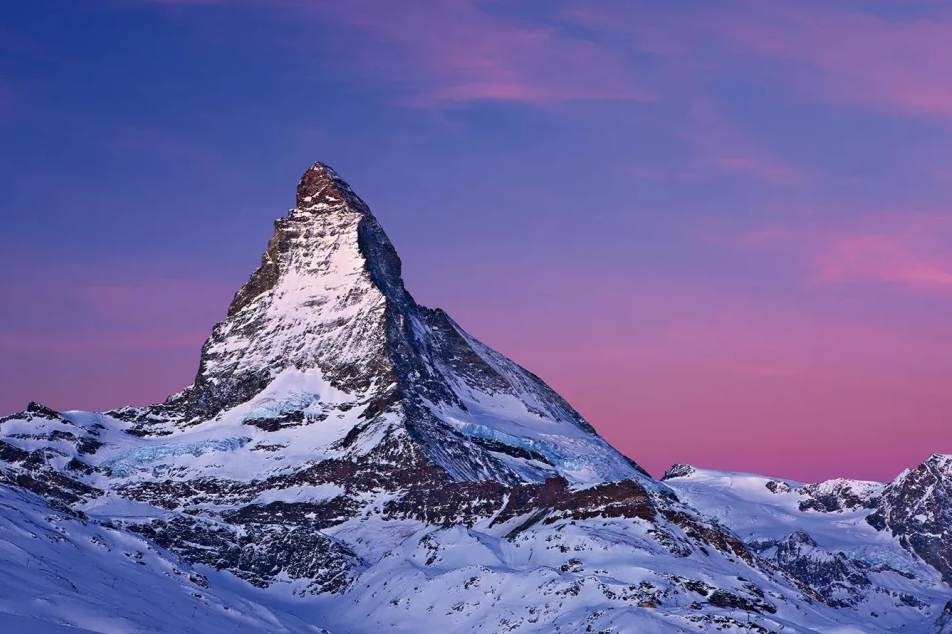
\includegraphics[width=0.8\linewidth]{fig/matterhorn.png}
    \caption{ยอดเขามัทเทอร์ฮอร์น (Matterhorn) ตั้งอยู่บนแนวของเทือกเขาแอลป์ ประเทศสวิตเซอร์แลนด์
        (เครดิตภาพ: https://www.myswitzerland.com)}
    \label{fig:matterhorn}
\end{figure}

Gradient เป็นกระบวนการทำซ้ำ (Iterative Process) โดยทําการขยับหรือกระโดดจากจุดหนึ่ง $(x^{k})$ ไปยังอีกจุดหนึ่ง $(x^{k+1})$
ในทิศทางที่ทําให้ค่าของฟังก์ชันมีค่าเพิ่มขึ้นหรือลดลงในปัญหาของการหาค่าสูงสุดหรือค่าต่ำสุดตามลำดับ จนกระทั่งได้ค่าที่เหมาะสมออกมา โดยสิ่งที่
Gradient Descent ทำในการหาพารามิเตอร์ที่เหมาะสมของฟังก์ชันก็คือการวนหาค่าที่ทำให้ Loss Function หรือค่าความคลาดเคลื่อนมีค่าน้อยที่สุด
โดยเราจะแทนความคลาดเคลื่อนหรือ Error ที่เกิดขึ้นด้วย $J$ (เช่นสมการที่ \eqref{eq:loss}) หรืออธิบายง่าย ๆ ก็คือหาจุดที่มี $J$ ต่ำที่สุด%
จากการคำนวณความชัน (Slope) ณ จุดที่เราอยู่แล้วพยายามหาเส้นทางในการขยับจุดไปในทิศทางตรงข้ามกับ Slope โดยให้ลองนึกภาพว่าเรา%
กำลังเดินขึ้นเขา เช่น ตามภาพที่ \ref{fig:matterhorn} โดยวิธีการเดินเพื่อไปให้ถึงจุดสูงสุดคือเราไต่ขึ้นตามทางที่ชันขึ้นเพื่อไปถึงจุดสูงสุดนั่นเอง
ถ้ายิ่งชันเท่าไหร่ก็มีแนวโน้มว่าเราเข้าใกล้จุดสูงสุดมากขึ้นเท่านั้น

Gradient Descent เป็นอัลกอริทึมที่ใช้หาจุดต่ำสุดหรือสูงสุดของฟังก์ชันซึ่งโดยส่วนมากเป็นฟังก์ชันรูปกรวยคว่ำ (Convex) แต่ถ้าลองดูตัวอย่างง่าย ๆ
เช่น ฟังก์ชันพาราโบลาหงายที่มีฟังก์ชันเป็น

\begin{equation}\label{eq:parabola}
    f(x) = x^2 - 4x
\end{equation}

\noindent เราจะสามารถหาอนุพันธ์ของสมการที่ \eqref{eq:parabola} ได้ง่าย ๆ ซึ่งจะได้ออกมาเป็นสมการที่อธิบายความชัน ดังนี้

\begin{align}\label{eq:parabola_slope}
    f'(x) & = \nabla f(x) \nonumber \\
          & = 2x - 4
\end{align}

%--------------------------
\subsection{Batch Gradient Descent}
\label{ssec:batch_grad}
\idxth{การเคลื่อนลงตามความชัน!แบทช์}
\idxen{Gradient Descent!Batch}
%--------------------------

คราวนี้เราลองมาดูกรณีที่ Loss Function นั้นเป็นแบบกรณีทั่วไปกันบ้าง โดยเรานิยามให้ Loss Function มีหน้าตาแบบนี้

\begin{align}\label{eq:batch_loss}
    J(\theta) & = J(\theta_0, \theta_1) \nonumber                                        \\
              & = \cfrac{1}{2m} \sum_{i=1}^m ((\theta_0 + \theta_1 x^{(i)}) - y^{(i)})^2
\end{align}

\noindent เราสามารถหา Gradient ได้ดังนี้

\begin{align}
    \nabla J (\theta) & = \begin{bmatrix} \cfrac{\partial J}{\partial \theta_0} \\ \cfrac{\partial J}{\partial
                                  \theta_1}\end{bmatrix}                 \\
                      & =  \begin{bmatrix} \frac{1}{m} \sum_{i=1}^{m} ((\theta_0 + \theta_1 x^{(i)}) - y^{(i)}) \\ \frac{1}{m}
                               \sum_{i=1}^{m} ((\theta_0 + \theta_1 x^{(i)}) - y^{(i)})x^{(i)}\end{bmatrix}
\end{align}

\noindent ซึ่งเราสามารถเขียนสมการในกรณีที่เราสนใจและอัพเดท $\theta$ ได้ดังนี้\footnote{สังเกตว่าเราใช้เครื่องหมาย $a := b$
    เพื่อบ่งบอกการดำเนินการ (Operation) ซึ่งเป็นการระบุค่าให้กับตัวแปรในโปรแกรมคอมพิวเตอร์}

\begin{equation}\label{eq:batch_grad}
    \theta := \theta - \alpha\nabla_\theta J(\theta)
\end{equation}

\noindent โดยสมการที่ \eqref{eq:batch_grad} นั้นคือ Batch Gradient Descent มีสัมประสิทธิ์ด้านหน้า $\nabla_\theta J$ ก็คือ
$\alpha$ คืออัตราเร็วในการเรียนรู้ \textit{Learning Rate} หรืออาจจะเรียกว่า \textit{Step Size} ก็ได้ โดยเรามักจะกำหนดให้ค่า
$\alpha$ มีค่ามากกว่าศูนย์ ซึ่งเป็นอัลกอริทึมแบบที่ง่ายที่สุดเพราะว่าใช้ข้อมูลทั้งหมดใน Training Set ในการฝึกสอนโมเดล ดังนั้นผู้อ่านน่าจะ%
พอเดาออกว่าถ้าหากเราใช้ Batch Gradient Descent กับชุดข้อมูลที่มีขนาดใหญ่มากนั้นก็จะใช้ระยะเวลานานในการฝึกสอนโมเดล นั่นก็เพราะว่า
Optimization แบบ Batch นั้นช้ามาก ด้านล่างคืออัลกอริทึมของ Batch Gradient Descent

\begin{algorithm}[H]
    \caption{อัลกอริทึมของ Batch Gradient Descent}
    \label{alg:batch_grad}
    \begin{algorithmic}
        \State Hyperparameter: learning rate $\alpha$, number of total iteration $n_\text{iter}$.
        \State Initialize $\theta$ randomly.
        \For{$i = 1$ to $n_\text{iter}$}
        \begin{equation*}
            \theta := \theta - \alpha\nabla_\theta J^{(j)}(\theta)
        \end{equation*}
        \EndFor
    \end{algorithmic}
\end{algorithm}

\noindent ตัวอย่างของโค้ดของ Batch Gradient Descent มีดังนี้

\begin{lstlisting}[style=MyPython]
for i in range(nb_epochs):
    params_grad = evaluate_gradient(
        loss_function, 
        data, 
        params
        )
    params = params - learning_rate * params_grad
\end{lstlisting}

%--------------------------
\subsection{Stochastic Gradient Descent}
\label{ssec:stochastic_grad}
\idxth{การเคลื่อนลงตามความชัน!สโตแคสติก}
\idxen{Gradient Descent!Stochastic}
%--------------------------

เพื่อแก้ปัญหาในกรณีที่ชุดข้อมูลมีขนาดใหญ่มากนั้น จึงได้มีการพัฒนาอัลกอริทึมแบบที่สองขึ้นมา เรียกว่า Stochastic Gradient Descent (SGD)
โดย SGD นี้เป็นวิธีที่ง่ายและไม่ซับซ้อนในการนำมาใช้ปรับค่าพารามิเตอร์ให้มีความเหมาะสม โดยในแต่ละครั้งของการคำนวณ Gradient เราจะทำ%
การสุ่มข้อมูลเพียงบางส่วนเพื่อใช้ในการอัพเดทค่าเท่านั้น ไม่ได้ใช้ข้อมูลทั้งหมดเหมือนในกรณี Batch โดยตามทฤษฎีแล้วได้มีการพิสูจน์ว่าเรา%
สามารถใช้ข้อมูลในปริมาณที่เล็กน้อยเพื่อใช้ในการอัพเดทพารามิเตอร์ในแต่ละครั้ง (Iteration) ได้โดยไม่ต้องนำข้อมูลทั้งหมดมาใช้ทีเดียว
ซึ่งในท้ายที่สุดแล้วการ Optimization ก็จะลู่เข้าสู่คำตอบที่ใกล้เคียงกัน ซึ่ง SGD นี้ถือว่ามีส่วนสำคัญต่อการฝึกสอนโมเดลที่มีพารามิเตอร์ที่เกี่ยวข้อง%
ในปริมาณที่เยอะมาก ๆ เช่น Neural Network การใช้ SGD สามารถลดปัญหาของการที่ Optimization นั้นติดหรือค้างอยู่ในจุดต่ำสุดสัมพันธ์%
ได้อีกด้วย ซึ่งการปรับค่าด้วย SGD นั้นจะใช้สมการดังต่อไปนี้

\begin{equation}\label{eq:sgd}
    \theta := \theta - \alpha\nabla_\theta J( \theta; x^{(i)}; y^{(i)})
\end{equation}

\noindent ด้านล่างคืออัลกอริทึมของ SGD

\begin{algorithm}[H]
    \caption{อัลกอริทึมของ Stochastic Gradient Descent}
    \label{alg:sgd}
    \begin{algorithmic}
        \State Hyperparameter: learning rate $\alpha$, number of total iteration $n_\text{iter}$.
        \State Initialize $\theta$ randomly.
        \For{$i = 1$ to $n_\text{iter}$}
        \State Sample $j$ uniformly from ${1,\ldots,n}$, and update $\theta$ by
        \begin{equation*}
            \theta := \theta - \alpha\nabla_\theta J^{(j)}(\theta)
        \end{equation*}
        \EndFor
    \end{algorithmic}
\end{algorithm}

\noindent ตัวอย่างของโค้ดของ Stochastic Gradient Descent มีดังนี้

\begin{lstlisting}[style=MyPython]
for i in range(nb_epochs):
    np.random.shuffle(data)
    for example in data:
        params_grad = evaluate_gradient(
            loss_function, 
            example, 
            params
            )
        params = params - learning_rate * params_grad
\end{lstlisting}

\vspace{1em}
\noindent นอกจากนี้แล้วในการฝึกสอนโมเดล Neural Network นั้น เรามักนิยมใช้ Stochastic Gradient Descent โดยด้านล่างคือ%
ตัวอย่างโค้ดของการเรียกใช้ Stochastic Gradient Descent (SGD) Optimizer ของ TensorFlow

\begin{lstlisting}[style=MyPython]
import tensorflow as tf

# Create an optimizer with the desired parameters
opt = tf.keras.optimizers.SGD(
    learning_rate=0.01,
    momentum=0.0,
    nesterov=False,
    name='SGD',
    **kwargs
)

# `loss` is a callable that takes no argument and 
# returns the value to minimize
loss = lambda: 3 * var1 * var1 + 2 * var2 * var2

# In graph mode, returns op that minimizes the loss 
# by updating the listed variables
opt_op = opt.minimize(loss, var_list=[var1, var2])
opt_op.run()

# In eager mode, simply call minimize to update 
# the list of variables
opt.minimize(loss, var_list=[var1, var2])
\end{lstlisting}

%--------------------------
\subsection{Mini-batch Stochastic Gradient Descent}
\label{ssec:minibatch_grad}
\idxth{การเคลื่อนลงตามความชัน!มินิ-แบทช์}
\idxen{Gradient Descent!Mini-batch}
%--------------------------

นอกเหนือจาก Batch และ Stochastic Gradient Descent แล้ว ยังมีอัลกอริทึมแบบที่สามที่เป็นการรวมข้อดีของทั้งสองอัลกอริทึมเข้าไว้ด้วยกัน
นั่นคืออัลกอริทึมที่ชื่อว่า Mini-batch Stochastic Gradient Descent โดยแนวคิดก็คือในทางปฏิบัตินั้นการคำนวณ Gradient ของ Batch
$(B)$ หลาย ๆ ครั้งสามารถทำพร้อมกันได้เพราะว่าในปัจจุบันเรามีเทคนิคการทำการคำนวณแบบขนาน (Parallelization) สำหรับการปรับค่า
$\theta$ ซึ่งจะเร็วกว่าการคำนวณ Gradient ของ $B$ แบบแยกกันทีละค่าแน่นอน ซึ่งการที่เราจะทำการคำนวณแบบพร้อม ๆ กันได้นั้นเราจะ%
ต้องมีการแบ่งข้อมูลของเราออกเป็นส่วนย่อย ๆ แล้วทำการคำนวณแยกกัน โดยมีสมการดังต่อไปนี้

\begin{equation}\label{eq:minibatch}
    \theta = \theta - \alpha\nabla_\theta J( \theta; x^{(i:i+n)}; y^{(i:i+n)})
\end{equation}

ในการคำนวณจริงนั้นเราจะต้องมีการปรับอัลกอริทึมเล็กน้อย โดยด้านล่างคืออัลกอริทึมของ Mini-batch SGD ซึ่งได้จากการปรับอัลกอริทึมของ SGD
แบบธรรมดา

\begin{algorithm}[H]
    \caption{อัลกอริทึมของ Mini-batch Stochastic Gradient Descent}
    \label{alg:minibatch}
    \begin{algorithmic}
        \State Hyperparameter: learning rate $\alpha$, batch size $B$, \# iteration $n_\text{iter}$.
        \State Initialize $\theta$ randomly.
        \For{$i = 1$ to $n_\text{iter}$}
        \State Sample $j$ uniformly from ${1,\ldots,n}$, and update $\theta$ by
        \State Sample $B$ examples $j_1,\ldots,j_B$ (without replacement) uniformly from $\{1,\ldots,n\}$,
        and update $\theta$ by
        \begin{equation*}
            \theta := \theta - \frac{\alpha}{B}\sum_{k=1}^B\nabla_\theta J^{(j_k)}(\theta)
        \end{equation*}
        \EndFor
    \end{algorithmic}
\end{algorithm}

\noindent ตัวอย่างของโค้ดของ Mini-batch Stochastic Gradient Descent มีดังนี้

\begin{lstlisting}[style=MyPython]
for i in range(nb_epochs):
    np.random.shuffle(data)
    for batch in get_batches(data, batch_size=50):
        params_grad = evaluate_gradient(
            loss_function, 
            batch, 
            params
            )
        params = params - learning_rate * params_grad
\end{lstlisting}

\vspace{1em}
\noindent $\bullet$ \textbf{สรุปเปรียบเทียบอัลกอริทึมของ Gradient Descent}

\begin{figure}[H]
    \centering
    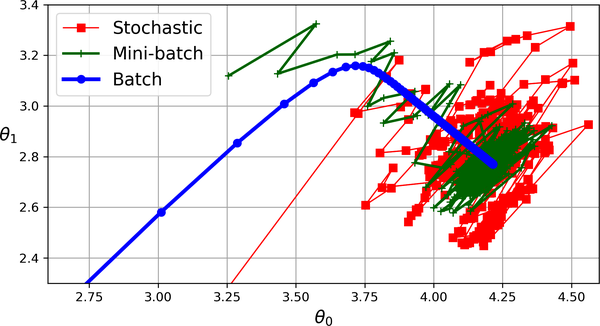
\includegraphics[width=0.9\linewidth]{fig/gradient_descent_path.png}
    \caption{วิถีของ Gradient Descent ในปริภูมิของพารามิเตอร์ (เครดิตภาพ: https://www.oreilly.com)}
    \label{fig:gradient_descent_path}
\end{figure}

ภาพที่ \ref{fig:gradient_descent_path} แสดงการเปรียบเทียบวิถี (Path) ของการขยับของ Gradient Descent ด้วยอัลกอริทึมที่ต่างกัน
ซึ่งแสดงอยู่บนปริภูมิพารามิเตอร์ โดยสรุปได้ว่าทั้งสามอัลกอริทึมนั้นให้ผลลัพธ์ที่เข้าใกล้จุดต่ำสุดแต่ว่าจริง ๆ แล้ว Batch Gradient Descent
นั้นหยุดอยู่ที่จุดต่ำสุดพอดีในขณะที่ Stochastic และ Mini-batch Gradient Descent นั้นจะขยับวนไปมาอยู่รอบ ๆ จุดต่ำสุดและยังคงขยับ%
ไปมาอยู่เรื่อย ๆ อย่างไรก็ตามเราจะต้องไม่ลืมว่าอัลกอริทึมแบบ Batch นั้นใช้ระยะเวลาในการขยับจากจุดหนึ่งไปยังอีกจุดหนึ่งที่นานมาก แต่อีกสอง%
อัลกอริทึมนั้นใช้เวลาน้อยกว่ามาก ซึ่งถ้าหากเราเลือกใช้อัลกอริทึม Stochastic หรือ Mini-batch ได้อย่างเหมาะสมแล้วทั้งสองอัลกอริทึมนี้ก็%
สามารถให้ผลลัพธ์ที่ลู่เข้า (Convergence) สู่จุดต่ำสุดได้เช่นเดียวกัน

โดยทั่วไปแล้วโมเดล Deep Learning นั้นจะมีการเรียนรู้ซึ่งอาศัยอัลกอริทึมตามด้านบนโดยทำตามขั้นตอนดังต่อไปนี้

\begin{enumerate}[topsep=0pt,noitemsep]
    \item กำหนด $h_\theta(x)$

    \item เขียนอัลกอริทึม Backpropagation เพื่อคำนวณ Gradient ของ Loss Function $J^{(j)}(\theta)$

    \item ทำการปรับ Loss Function โดยใช้ SGD หรือ Mini-batch SGD หรือใช้อัลกอริทึมอื่น เช่น Normal Equation หรือ SVD
\end{enumerate}

นอกจากนี้แล้วอีกสิ่งหนึ่งที่เราต้องคำนึงถึงก็คือ Learning Rate ซึ่งเป็นค่าอัตราเร็วของการเรียนรู้ โดยพารามิเตอร์ตัวนี้มีผลทั้งในเชิงประสิทธิภาพ%
ของอัลกอริทึมที่ใช้ในการปรับให้การ Optimization นั้นลู่เข้าและมีผลต่อความเร็วหรือความสิ้นเปลืองในการปรับค่าด้วย

\begin{figure}[H]
    \centering
    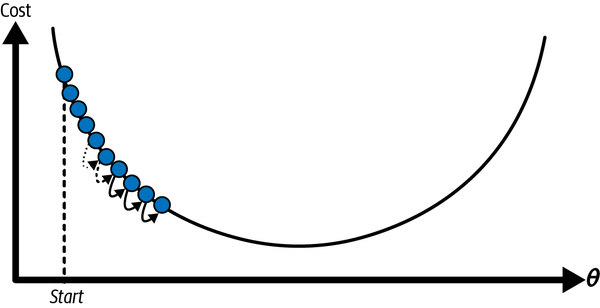
\includegraphics[width=0.8\linewidth]{fig/learning_rate_small.png}
    \caption{แสดงค่าคลาดเคลื่อน (Error หรือ Cost) เทียบกับการเปลี่ยนแปลงของการเรียนรู้ในกรณีที่กำหนดให้ Learning Rate นั้นมี%
        ที่น้อยมาก ๆ (เครดิตภาพ: https://www.oreilly.com)}
    \label{fig:learning_rate_small}
\end{figure}

\begin{figure}[H]
    \centering
    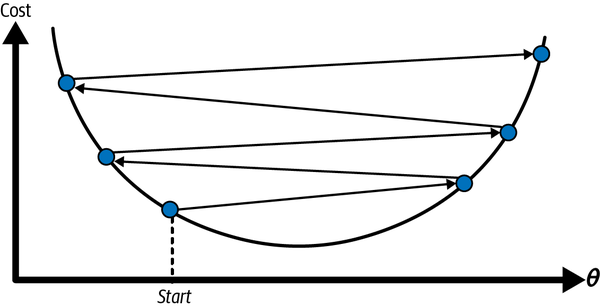
\includegraphics[width=0.8\linewidth]{fig/learning_rate_high.png}
    \caption{แสดงค่าคลาดเคลื่อน (Error หรือ Cost) เทียบกับการเปลี่ยนแปลงของการเรียนรู้ในกรณีที่กำหนดให้ Learning Rate นั้นมี%
        ที่สูงมาก ๆ (เครดิตภาพ: https://www.oreilly.com)}
    \label{fig:learning_rate_high}
\end{figure}

ภาพที่ \ref{fig:learning_rate_small} และ \ref{fig:learning_rate_high} แสดงความสามารถในการขยับหรือปรับค่าของการทำ
Gradient Descent จากจุดหนึ่งไปยังอีกจุดหนึ่งโดยใช้อัตราเร็วในการเรียนรู้ที่มีค่าน้อย ๆ และค่าสูง ๆ ตามลำดับ โดยเราสามารถสรุปได้ว่าในกรณี%
ที่เราใช้อัตราการเรียนรู้ที่มีค่าน้อยเกินไปนั้นจะเป็นการขยับจุดแบบช้ามาก ๆ และการขยับไปในแต่ละจุดนั้นจะเป็นแบบก้าวสั้น ๆ แต่ก็ให้ผลลัพธ์ที่มีความ%
แม่นยำและค่อย ๆ ขยับจุดเข้าไปใกล้จุดต่ำสุดตามที่ต้องการ ซึ่งจะตรงข้ามกับกรณีที่ใช้อัตราการเรียนรู้ที่สูงเกินไปนั่นก็คือการขยับจุดนั้นเป็นไปอย่าง%
รวดเร็ว และระยะห่างระหว่างจุดหรือขนาดของก้าวแต่ละก้าวนั้นจะกว้างกว่ามาก แต่จะพบว่าการปรับค่าเข้าไปหาจุดต่ำสุดนั้นจะทำได้ไม่ค่อยดีเพราะจะ%
เป็นการขยับจุดที่เร็วเกินไปทำให้เกิดการวนซ้ำไปซ้ำมารอบ ๆ จุดต่ำสุดและทำให้ลู่เข้าได้ยากเพราะว่าหาจุดต่ำสุดจริง ๆ ไม่เจอเสียที

สรุปคือเราควรจะต้องกำหนดอัตราเร็วของการเรียนรู้ให้มีความเหมาะสม ถ้าหากอัตราการเรียนรู้ช้าเกินไปก็จะใช้เวลานาน แต่ถ้าหากอัตราการเรียนรู้เร็ว%
เกินไปก็จะทำให้การปรับค่านั้นได้ผลลัพธ์ที่ไม่แม่นยำ นอกจากนี้แล้วเราไม่มีกฎตายตัวในการหาค่าอัตราเร็วในการเรียนรู้ที่ดีที่สุด ดังนั้นการเลือกค่า%
อัตราเร็วการเรียนรู้หรือ Learning Rate นั้นจึงเป็น Art อย่างหนึ่งของการทำ Deep Learning ซึ่งเป็น Hyperparameter ที่สำคัญมากจนถึง%
กับมีการกล่าวว่า \enquote{ถ้าหากจะต้องเลือกปรับ Hyperparameter ได้เพียงแค่หนึ่งตัว สิ่งที่เราควรจะต้องเลือกนั้นก็คือ Learning Rate}%
\footnote{ค่า Default ของ Learning Rate ของ Adam Optimizer ที่ถูกกำหนดไว้ใน TensorFlow คือ 0.001}

%--------------------------
\section{โครงข่ายประสาทเทียม}
\label{sec:nn}
\idxboth{โครงข่ายประสาทเทียม}{Neural Network}
\idxen{Artificial Neural Network}
%--------------------------

โครงข่ายประสาทเทียม (Neural Network) ถือว่าเป็นโมเดล ML แบบหนึ่งที่มีประสิทธิภาพสูงมากและเป็นสิ่งที่พลิกโฉมหน้าประวัติศาสตร์ของวงการ%
ปัญญาประดิษฐ์เลยก็ว่าได้ ตามที่ได้อธิบายไว้คร่าว ๆ ในหัวข้อ \ref{ssec:ann} แล้วว่า Neural Network นั้นเป็นการเลียนแบบการทำงานของ%
สมองมนุษย์ ซึ่งในช่วงยุคต้นของการพัฒนาเทคนิคนี้นั้นมีจุดประสงค์คือการแก้ปัญหาแบบเดียวกับที่สมองมนุษย์สามารถทำได้ แต่เมื่อเวลาผ่านไป%
จุดประสงค์ของการสร้าง Neural Network ก็ได้เปลี่ยนไปเป็นการทำงานที่เฉพาะเจาะจงมากขึ้น และมีการพัฒนาให้สามารถทำงานหรือแก้ปัญหาให้%
ดีกว่ามนุษย์เสียอีก ซึ่งเป็นการแทนจุดประสงค์เดิมในการสร้างสมองเทียม โดยในปัจจุบันมีการประยุกต์ใช้โ Neural Network กับงานหลากหลายรูปแบบ
เช่น คอมพิวเตอร์วิทัศน์ (Computer Vision), การเรียนรู้เสียง (Voice Learning และ Recognition), การแปลภาษา (Translation),
การกรองเนื้อหาโซเชียลมีเดีย, การเล่นเกม, การวินิจฉัยโรค และกิจกรรมที่ไม่คิดว่าปัญญาประดิษฐ์จะทำได้ เช่น การวาดภาพ, การประพันธ์เพลง
และการประพันธ์บทกวี

Neural Network ที่พบได้ทั่วไปจะมีลักษณะคือประกอบไปด้วยชั้นของเซลล์ประสาทเทียม (Neural Layer) คือ ชั้นที่รับข้อมูลขาเข้าเรียกว่าชั้นอินพุต
(Input Layer), ชั้นที่สร้างข้อมูลขาออกเรียกว่าชั้นเอาต์พุต (Output Layer) และชั้นอื่น ๆ ที่อยู่ตรงกลางระหว่างชั้นอินพุตและชั้นเอาต์พุตที่มี%
ส่วนในการช่วยทำการประมวลผลอยู่ภายในเรียกว่าชั้นซ่อน (Hidden Layer) ซึ่งใน Neural Network อาจมี Hidden Layer ได้หลายชั้น
นอกจากนี้เราสามารถแบ่งโครงสร้างพื้นฐานตามการไหล (Flow) ของข้อมูลได้ดังต่อไปนี้
\idxboth{ชั้นของเซลล์ประสาทเทียม}{Neural Layer}
\idxboth{ชั้นของเซลล์ประสาทเทียม!ชั้นอินพุต}{Neural Layer!Input Layer}
\idxboth{ชั้นของเซลล์ประสาทเทียม!ชั้นเอาต์พุต}{Neural Layer!Output Layer}
\idxboth{ชั้นของเซลล์ประสาทเทียม!ชั้นซ่อน}{Neural Layer!Hidden Layer}

\begin{itemize}[topsep=0pt,noitemsep]\setlength\itemsep{0.5em}
    \item แบบป้อนไปข้างหน้า (Feed-forward) เป็น Neural Network ที่ข้อมูลจะมีการไหลหรือส่งต่อไปในทิศทางเดียวจาก Input Layer
          ไปยัง Hidden Layer และ Output Layer ตามลำดับ การเชื่อมโยงจะถูกกำหนดขึ้นระหว่างชั้นที่ติดกันโดยจะมีการเชื่อมโยงระหว่างเซลล์%
          ประสาทเทียม (Neuron) ทุกตัว จากชั้นหนึ่ง ๆ ไปยังเซลล์ประสาทเทียมทุกตัวในชั้นต่อไป ในบางสถาปัตยกรรมอาจมีการเชื่อมโยงข้ามชั้นก็ได้
          นอกจากนี้แล้วรูปแบบของ Neural Network ประเภทนี้ยังจัดแบ่งได้เป็นสองแบบย่อยคือ แบบมีชั้นของเซลล์ประสาทชั้นเดียว และแบบมีชั้น%
          ของเซลล์ประสาทหลายชั้น
          \idxboth{โครงข่ายประสาทเทียม!แบบป้อนไปข้างหน้า}{Neural Network!Feed-forward}

    \item แบบมีการป้อนไปเวียนกลับ (Recurrent) เป็น Neural Network ที่การเชื่อมโยงที่ถูกกำหนดขึ้นระหว่างเซลล์ประสาทเทียมในชั้น%
          หนึ่ง ๆ นั้นย้อนกลับไปยังชั้นอื่น ๆ ก่อนหน้านั้นได้หรือแม้แต่ภายในชั้นเดียวกันเองโดยผ่านการวนลูปรอบ ๆ เซลล์ประสาทนั้น ๆ โดยการไหล%
          ของข้อมูลนั้นสามารถเกิดได้สองทิศทาง ทั้งทิศทางที่ไปข้างหน้าและย้อนกลับ สถาปัตยกรรมแบบนี้ยังมีชื่อเรียกอีกชื่อว่า Feedback Neural
          Network
          \idxboth{โครงข่ายประสาทเทียม!แบบป้อนเวียนกลับ}{Neural Network!Recurrent}
\end{itemize}

สำหรับในหัวข้อนี้เราจะมาดูการเรียนรู้เชิงลึก (Deep Learning) รูปแบบที่มาตรฐานที่สุดคือการเรียนรู้แบบมีผู้สอนด้วยโมเดลแบบไม่เป็นเชิงเส้น
(Supervised Learning with Nonlinear Model) นอกจากนี้ Neural Network ยังมีสถาปัตยกรรมที่หลากหลายซึ่งผู้อ่านสามารถศึกษาได้%
ในหัวข้อที่ \ref{sec:arch_nn}

%--------------------------
\section{การแผ่กระจายการเรียนรู้}
\idxboth{การแผ่กระจายการเรียนรู้}{Learning Propagation}
%--------------------------

การแผ่กระจายการเรียนรู้ (Learning Propagation) เป็นขั้นตอนการเรียนรู้ของโมเดล Neural Network ที่เลียนแบบการทำงานของสมอง

\begin{figure}[H]
    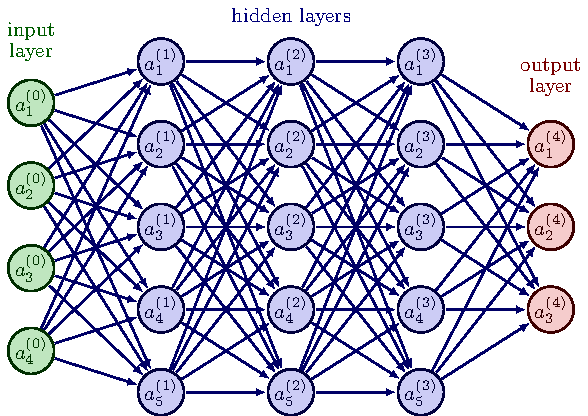
\includegraphics[width=\linewidth]{fig/dense_neural_net.pdf}
    \caption{โครงข่ายประสาทแบบสมบูรณ์ (Dense Neural Network) มี Notation $a^{(j)}_{i}$ แทนข้อมูลของหน่วยเรียนรู้หรือ%
        นิวรอนที่ $i$ ของชั้นที่ $j$ โดยชั้นที่ 1 กับชั้นที่ 4 ของตัวอย่าง Neural Network นี้คือชั้นอินพุตและชั้นเอาต์พุตตามลำดับ}
    \label{fig:dense_neural_net}
\end{figure}

จะเห็นได้ว่าไดอะแกรมด้านบนนั้นมีความซับซ้อนมาก ซึ่งจริง ๆ แล้วถ้าหากเราจะมาทำความเข้าใจองค์ประกอบของ Neural Network นั้น เราควร%
พิจารณากรณีง่าย ๆ ด้วยโครงสร้างแบบเล็ก ๆ ก่อน ตามภาพที่ \ref{fig:nn_layer} ซึ่งเป็นชั้นการเรียนรู้ (Learning Layer) ประกอบไปด้วย
3 ส่วน ดังนี้

\begin{description}
    \item[Input Layer] ชั้นอินพุต เก็บข้อมูลที่เราจะนำมาใช้ในการฝึกสอนโมเดล โดยในแต่ละหน่วยประสาท (Neuron หรือ Learning Unit
        หรือ Node) จะเป็นตัวที่เก็บคุณลักษณ์ที่อยู่ในข้อมูล เช่น ความยาวพันธะหรือจำนวนเวเลนซ์อิเล็กตรอนของอะตอม

    \item[Hidden Layer] ชั้นที่ถูกซ่อนไว้ เป็นชั้นที่อยู่ระหว่างชั้นอินพุตและชั้นเอาต์พุต โดยข้อมูลที่ถูกส่งมาจากชั้นก่อนหน้า (ในที่นี้คือชั้นอินพุต)
        จะถูกนำไปผ่านฟังก์ชันกระตุ้น (Activation Function) ในชั้นนี้ และหลังจากนั้นจะถูกส่งออกไปชั้นต่อไป (ในที่นี้คือชั้นเอาต์พุต)

    \item[Output Layer] ชั้นเอาต์พุต เป็นชั้นสุดท้ายของ Neural Network โดยจะรับข้อมูลหรืออินพุตมาจากชั้นก่อนหน้าซึ่งเป็น Hidden
        Layer โดยในชั้นนี้อาจจะมีการนำฟังก์ชันกระตุ้นมาใช้หรือไม่ใช้ก็ได้
\end{description}

\begin{figure}[H]
    \centering
    \begin{subfigure}{0.5\textwidth}
        \centering
        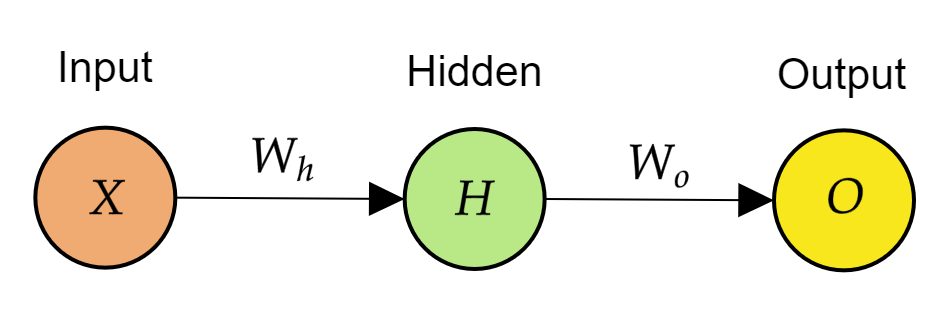
\includegraphics[width=0.9\linewidth]{fig/nn_layer.png}
        \caption{ชั้นการเรียนรู้ (Learning Layer)}
        \label{fig:nn_layer}
    \end{subfigure}%
    \begin{subfigure}{0.5\textwidth}
        \centering
        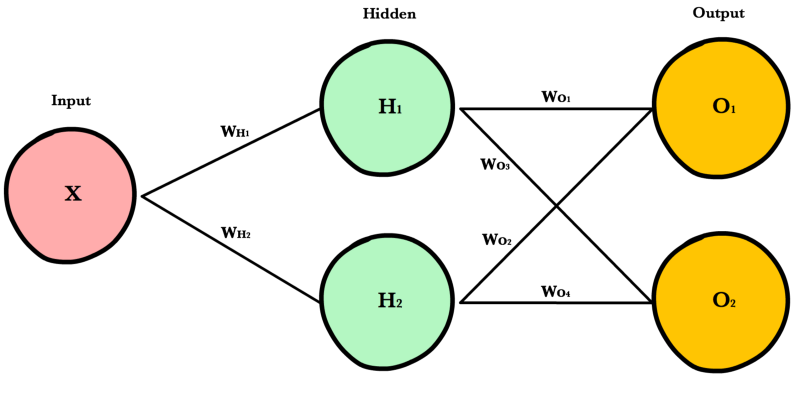
\includegraphics[width=0.9\linewidth]{fig/nn_w_matrices.png}
        \caption{โครงข่ายแบบค่าน้ำหนักหลายตัว}
        \label{fig:nn_w_matrices}
    \end{subfigure}
    \caption{ตัวอย่างของโครงข่ายประสาทแบบง่าย}
    \label{fig:nn_layer_w}
\end{figure}

โดยเราสามารถใช้โค้ดต่อไปนี้ในการสร้าง Neural Network แบบง่าย ๆ ได้

\begin{lstlisting}[style=MyPython]
def relu(z):
    return max(0,z)

def feed_forward(x, Wh, Wo):
    # Hidden layer
    Zh = x * Wh
    H = relu(Zh)

    # Output layer
    Zo = H * Wo
    output = relu(Zo)
    return output
\end{lstlisting}

\vspace{1em}
เมื่อเราพิจารณาภาพที่ \ref{fig:nn_w_matrices} ซึ่งมีความซับซ้อนมากขึ้นโดยมีการเพิ่มจำนวน Neuron เข้าไปในชั้น Hidden Layer และ
Output Layer เราจะพบว่าค่าน้ำหนักที่ถูกคำนวณออกมาจากชั้น Input จะถูกส่งไปยังชั้น Hidden และค่าน้ำหนักที่ออกมาจากชั้น Hidden ก็ถูก%
ส่งต่อไปยังชั้น Output ตามลำดับ โดยจะเห็นว่าทุก ๆ Neuron ของชั้นที่ถูกติดกันนั้นจะมีการแลกเปลี่ยนกันทุก Neuron โดยสมการที่ใช้ในการคำนวณ%
หาเอาต์พุตของแต่ละ Neuron มีดังนี้

\noindent $\bullet$ อินพุต 1 ตัว
\begin{align}\label{eq:nn_one_input}
    Z & = Input \cdot Weight \nonumber \\
      & = X W
\end{align}

\noindent $\bullet$ อินพุตมากกว่า 1 ตัว
\begin{align}\label{eq:nn_multi_input}
    Z & = \sum_{i=1}^{n}x_i w_i \nonumber \\
      & = x_1 w_1 + x_2 w_2 + x_3 w_3
\end{align}

เราจะสังเกตได้ว่าสมการที่ \eqref{eq:nn_one_input} และ \eqref{eq:nn_multi_input} เป็นสมการที่เหมือนกับที่เราใช้ใน Linear
Regression เป๊ะ ๆ เลย ซึ่งจริง ๆ แล้ว Neural Network ที่มีจำนวน Neuron แค่ 1 อันนั้นคือ Linear Regression เลย แต่สิ่งที่ต่างกันก็คือ
Neural Network จะมีกระบวนที่เกี่ยวข้องกับค่าน้ำหนักและฟังก์ชันกระตุ้นด้วย สำหรับการกำหนดค่าน้ำหนักในช่วงเริ่มต้นของการฝึกสอนนั้นเราสามารถ%
กำหนดค่าได้โดยใช้การสุ่มค่าตามตัวอย่างโค้ดดังต่อไปนี้

\begin{lstlisting}[style=MyPython]
import numpy as np

INPUT_LAYER = 1
HIDDEN_LAYER = 2
OUTPUT_LAYER = 2

def init_weights():
    Wh = np.random.randn(INPUT_LAYER, HIDDEN_LAYER) \
            * np.sqrt(2.0/INPUT_LAYER)
    Wo = np.random.randn(HIDDEN_LAYER, OUTPUT_LAYER) \
            * np.sqrt(2.0/HIDDEN_LAYER)
\end{lstlisting}

\vspace{1em}
\noindent และเรามักจะกำหนดค่าเริ่มต้นของความโน้มเอียง (Bias) ด้วยค่าน้อย ๆ เช่น 0.1 หรือ 0.2 ดังตัวอย่างต่อไปนี้

\begin{lstlisting}[style=MyPython]
def init_bias():
    Bh = np.full((1, HIDDEN_LAYER), 0.1)
    Bo = np.full((1, OUTPUT_LAYER), 0.1)
    return Bh, Bo
\end{lstlisting}

%--------------------------
\subsection{การแผ่กระจายแบบไปข้างหน้า}
\label{ssec:forward_prop}
\idxboth{การแผ่กระจายการเรียนรู้!การแผ่กระจายแบบไปข้างหน้า}{Propagation!Forward Propagation}
%--------------------------

ในขั้นเริ่มต้นของการฝึกสอนโมเดล Neural Network นั้น โมเดลจะยังไม่มีพารามิเตอร์ที่ถูกต้อง ดังนั้นเราจึงต้องสุ่มค่าเริ่มต้นของพารามิเตอร์ขึ้นมาก่อน
หลังจากนั้นจึงทำ Forward Propagation รอบที่หนึ่งแล้วก็เปรียบเทียบผลการทำนายกับคำตอบ (Output) ที่โมเดลทราบก่อนหน้านั้นแล้ว
ขั้นตอนต่อมาคือการปรับพารามิเตอร์ที่สำคัญอีกสองตัวนั่นคือน้ำหนัก (Weight) และความอคติหรือความโน้มเอียง (Bias) ให้มีค่าที่ถูกต้อง
ซึ่งในขั้นตอนนี้เราจะใช้กระบวนการที่ตรงข้ามกันที่เรียกว่า Backward propagation (หรือ Backpropagation) โดยการทำ Propagation
ทั้งสองแบบพร้อม ๆ กันครบหนึ่งรอบนั้นจะเรียกว่า 1 Epoch แต่ต้องระวังนะครับว่า Epoch, Batch Size และ Iteration นั้นมีความหมายต่างกัน
โดยความแตกต่างมีดังนี้

\begin{description}[font=$\bullet$~\normalfont\scshape\bfseries\color{blue!50!black}]
    \item[1 Epoch] การทำ Forward และ Backward Propagation 1 ครั้ง

    \item[Batch Size] จำนวนของข้อมูลที่ใช้ในการฝึกสอนในการทำ Forward และ Backward Propagation 1 รอบ

    \item[Iteration] จำนวนของรอบในการฝึกสอน ซึ่งแต่ละรอบจะใช้ Batch Size ที่ถูกกำหนดไว้ก่อนการฝึกสอน
\end{description}

เพื่อให้เห็นภาพมากขึ้น เราลองมาดูตัวอย่างกันครับ เช่น ถ้าเรามีจำนวนข้อมูลในการฝึกสอน 1,000 ข้อมูลและกำหนด Batch Size เป็น 500
จะได้ว่าโมเดลของเราจะใช้ 2 Iterations สำหรับการฝึกสอน 1 Epoch

\begin{figure}[H]
    \centering
    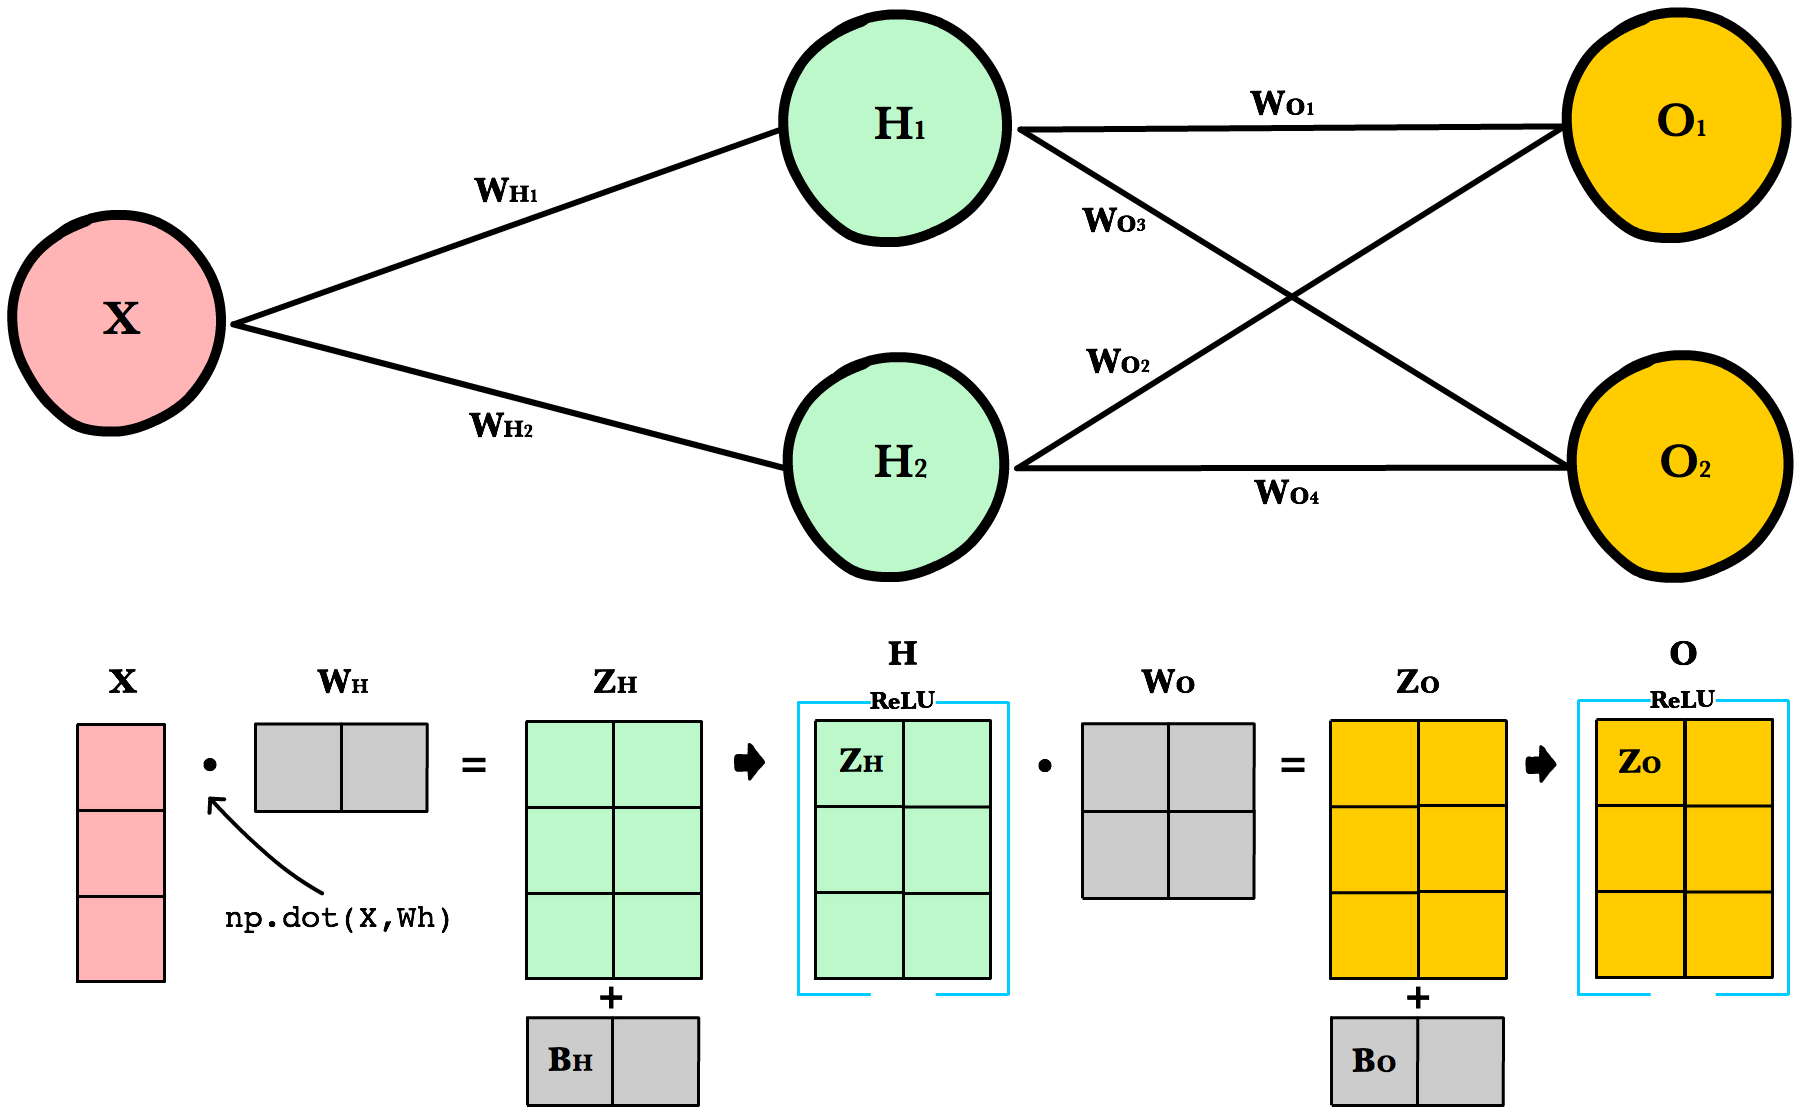
\includegraphics[width=0.9\linewidth]{fig/nn_feedforward_matrices.png}
    \caption{แผนภาพการดำเนินการคูณเมทริกซ์อินพุนด้วยเมทริกซ์น้ำหนัก}
    \label{fig:nn_ff_mat}
\end{figure}

\begin{figure}[H]
    \centering
    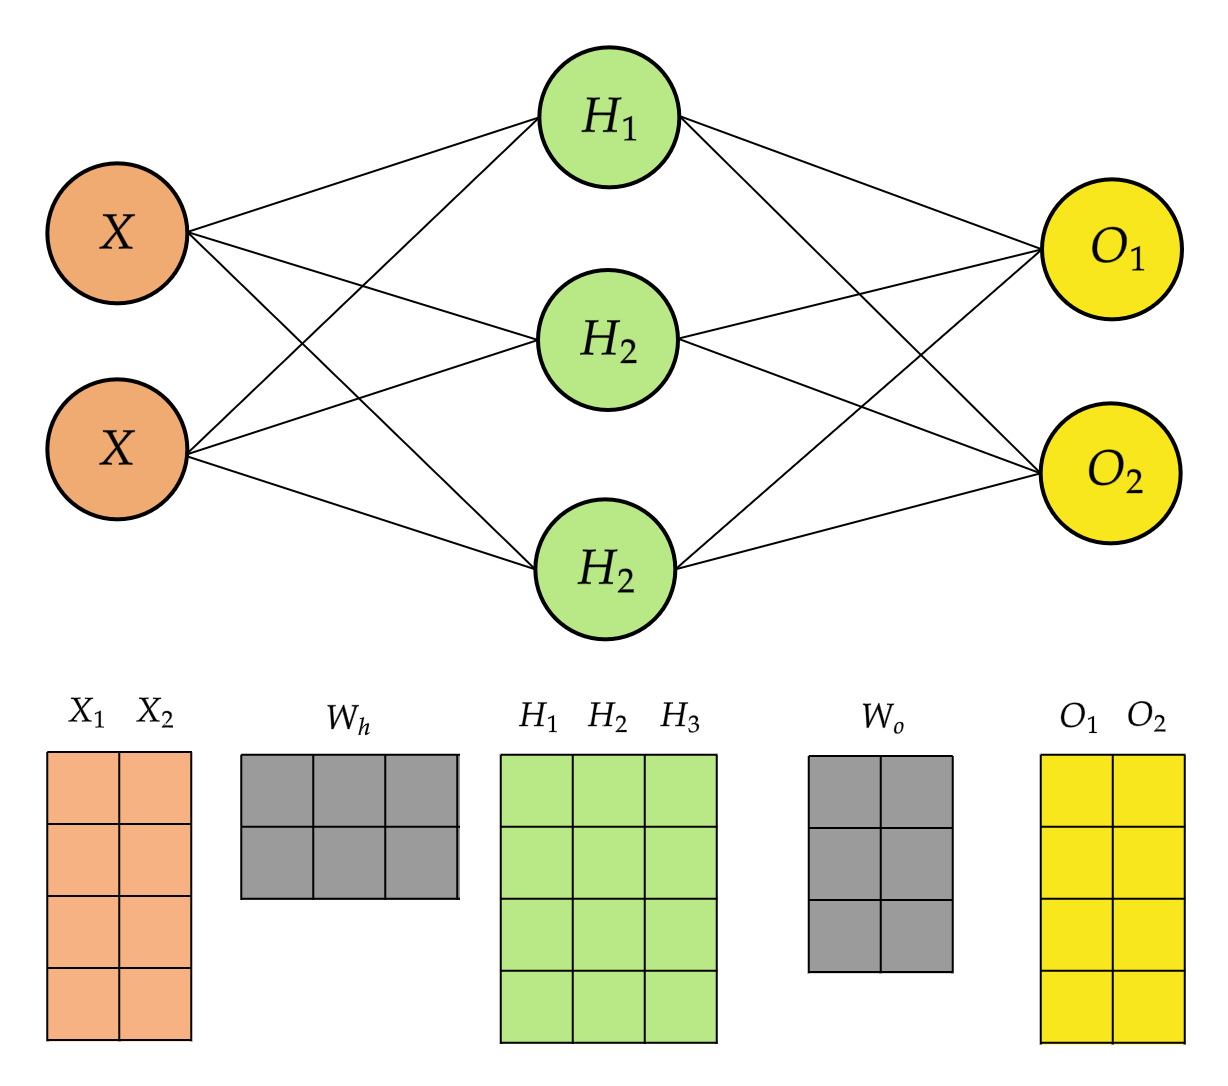
\includegraphics[width=0.8\linewidth]{fig/nn_feedforward_dyn_resizing.png}
    \caption{แผนภาพขนาดของเมทริกซ์ที่สามารถปรับขนาดได้แบบไดนามิกส์}
    \label{fig:nn_ff_dyn_resize}
\end{figure}

\begin{figure}[H]
    \centering
    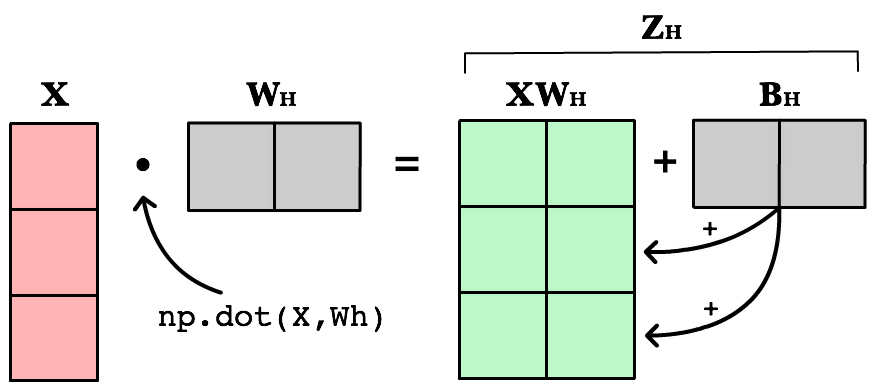
\includegraphics[width=0.8\linewidth]{fig/nn_feedforward_matrix_weighted_input.png}
    \caption{แผนภาพการดำเนินการคูณเมทริกซ์น้ำหนักและการเพิ่มความโน้มเอียง}
    \label{fig:nn_ff_mat_w}
\end{figure}

%--------------------------
\subsection{การแผ่กระจายแบบย้อนกลับ}
\label{ssec:backprop}
\idxboth{การแผ่กระจายการเรียนรู้!การแผ่กระจายแบบย้อนกลับ}{Propagation!Backpropagation}
%--------------------------

การแผ่กระจายแบบย้อนกลับ (Backpropagation) เป็นหัวใจหลักของ Deep Learning เลยก็ว่าได้\footnote{ใน Neural Network เราเน้นที่
    Deep Learning} นั่นก็เพราะว่าถ้า Neural Network ที่เราสร้างขึ้นนั้นมีแต่การเรียนรู้แบบแผ่ไปข้างหน้าโดยที่พารามิเตอร์ของโมเดลไม่มีการถูกปรับ
(Optimization) ให้เหมาะสมนั้น ความสามารถในการทำนายค่าก็จะไม่เพิ่มขึ้น ดังนั้นถ้าหากเราต้องการเพิ่มความสามารถในการเรียนรู้ของโมเดล
การแผ่กระจายย้อนกลับ (เรียกสั้น ๆ ว่า Backprop) นั้นจึงจำเป็นมาก เพราะการทำ Backprop นั้นเป็นการปรับค่า Weight โดยการเทียบกับ Loss
Function ของเรา ซึ่ง Loss Function นี้เองที่เป็นตัวบอกความแตกต่างระหว่างค่าเอาต์พุตหรือค่าที่เราทำนาย (Prediction) กับค่าอ้างอิง
(Reference) ดังนั้นถ้าหากเราต้องการที่จะปรับค่า Weight เพื่อให้มี Loss ที่น้อยลงเรื่อย ๆ เราสามารถทำได้โดยการหาอนุพันธ์ของ Loss
เทียบกับ Weight แต่ว่าใน Neural Network นั้นมี Weight หลายค่ามาก ดังนั้นเราจึงจำเป็นต้องใช้กฎลูกโซ่เข้ามาช่วยในการหาอนุพันธ์หลายตัวแปร
\idxboth{กฎลูกโซ่}{Chain Rule}

\begin{figure}[H]
    \centering
    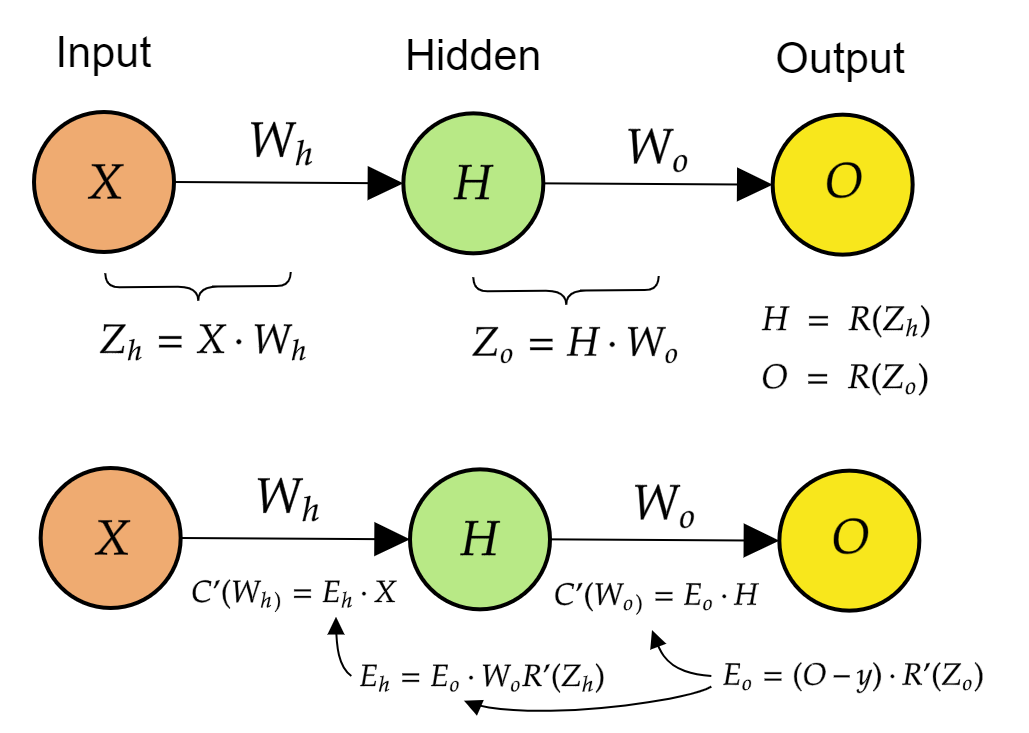
\includegraphics[width=0.8\linewidth]{fig/nn_backprop.png}
    \caption{การคำนวณการแผ่กระจายแบบย้อนกลับจากชั้นเอาต์พุตไปยังชั้นอินพุน}
    \label{fig:nn_bp}
\end{figure}

สำหรับการหาอนุพันธ์ของ Loss เทียบกับ Weight นั้นเราสามารถกระจายอนุพันธ์ออกมาให้อยู่ในรูปที่มี Weight จากแต่ละชั้น (Layer) ได้
เมื่อเราทำการหาอนุพันธ์นั้นเราจะต้องทำการหาของ Weight ที่อยู่ในชั้นท้ายสุดไล่ไปหาชั้นแรกสุด (ดูตามภาพที่ \ref{fig:nn_bp})
นั่นจึงเป็นเหตุผลที่เราเรียกการแผ่กระจายแบบนี้ว่าการแผ่กระจายย้อนกลับเพราะว่าเราทำการปรับ Weight ของ Hidden Layer จากหลังไปหน้านั่นเอง

\begin{algorithm}[ht]
    \caption{อัลกอริทึมของ Backpropagation สำหรับ Neural Network ซึ่งแสดงด้วย Computation Graph $G = (V,E)$.}
    \label{alg:backprop}
    \begin{enumerate}
        \item For a sample $(x_n ,y^*_n)$, propagate the input $x_n$ through the
              network to compute the outputs $(v_{i_1}, \ldots, v_{i_{|V|}})$ (in topological order).
              %\begin{enumerate}[(a)]
              %  \item Given a topological sort $V = (v_{i_1},\ldots,v_{i_{|V|}})$,
              %  sequentially compute the layers' outputs, also denoted by $v_{i_j}$.
              %  \item Then $y(x_n;w) = v_{i_{|V|}}$ is the network's output.
              %\end{enumerate}

        \item Compute the loss $\mathcal{L}_n := \mathcal{L}(v_{i_{|V|}}, y_n^*)$
              and its gradient
              \begin{align}
                  \frac{\partial \mathcal{L}_n}{\partial v_{i_{|V|}}}.
              \end{align}

        \item For each $j = |V|,\ldots,1$ compute
              \begin{align}
                  \frac{\partial \mathcal{L}_n}{\partial w_j} =
                  \frac{\partial \mathcal{L}_n}{\partial v_{i_{|V|}}} \prod_{k = j + 1}^{|V|}
                  \frac{\partial v_{i_k}}{\partial v_{i_{k - 1}}}
                  \frac{\partial v_{i_j}}{\partial w_j}.
              \end{align}
              where $w_j$ refers to the weights in node $i_j$.
    \end{enumerate}
\end{algorithm}

สำหรับผู้อ่านที่สนใจอัลกอริทึมของ Backprop สามารถศึกษาเพิ่มเติมได้ที่หัวข้อ \ref{alg:backprop}

%--------------------------
\section{ฟังก์ชันกระตุ้น}
\label{sec:act_func}
\idxboth{ฟังก์ชันกระตุ้น}{Activation Function}
%--------------------------

ฟังก์ชันกระตุ้น (Activation Function) หรือเรียกอีกชื่อว่า ฟังก์ชันการส่งต่อ (Transfer Function) เป็นหนึ่งใน Hyperparameters
ที่สำคัญมาก ๆ ของ Neural Network นั่นก็เพราะว่าฟังก์ชันกระตุ้นนี้จะทำหน้าที่ในการปรับให้ฟังก์ชันที่ใช้อธิบายความสัมพันธ์ระหว่างข้อมูล $x$
และ $y$ นั้นมีความไม่เป็นเส้นตรง (Nonlinearity) อธิบายง่าย ๆ ก็คือ Neural Network ที่ไม่มีการใช้ฟังก์ชันกระตุ้นก็จะไม่ต่างอะไรจากโมเดล
Linear Regression แบบเส้นตรงนั่นเอง โดยสิ่งที่ฟังก์ชันกระตุ้นทำก็คือจะทำการคำนวณค่าของเอาต์พุตออกมา ซึ่งรูปแบบของฟังก์ชันกระตุ้น%
ก็จะมีหลากหลายรูปแบบ เนื่องจากปัญหาของข้อมูลในโลกความเป็นจริงมีลักษณะเป็นแบบสมการเส้นตรงน้อยมาก ฟังก์ชันกระตุ้นจึงเป็นเปรียบเสมือน%
เป็นเจ้าหน้าที่ที่คอยตัดสินใจว่าหน่วยเรียนรู้ (Node) ควรจะถูกกระตุ้นเพื่อให้เกิดการเรียนรู้หรือไม่ โดยพิจารณาจากค่าผลรวมของอินพุต, ค่า Weight,
และค่า Bias โดยฟังก์ชันกระตุ้นถูกนำไปใช้ทั้งกับ Node ใน Hidden Layer และใน Output Layer ซึ่ง Node ในทั้งสองชั้นนี้อาจจะใช้ฟังก์ชัน%
กระตุ้นที่เหมือนหรือต่างกันก็ได้ ขึ้นอยู่กับความสามารถและพฤติกรรมของการเรียนรู้ของชั้นนั้น ๆ
\idxboth{ฟังก์ชันการส่งต่อ}{Transfer Function}

โดยส่วนมากแล้วเรามักจะใช้ฟังก์ชันกระตุ้นแบบไม่เป็นเชิงเส้นกับ Hidden Layer เหตุผลก็คือเนื่องจากว่าใน Hidden Layer จะมีการคำนวณแบบ%
การรวมเชิงเส้น ถ้าฟังก์ชันกระตุ้นของ Hidden Layer มีการคำนวณแบบเชิงเส้นอีกก็จะเป็นการเรียนรู้การทำงานที่ซ้ำซ้อนกับการคำนวณแบบการรวม%
เชิงเส้นใน Output Layer และจะส่งผลให้ผลลัพธ์นั้นเทียบเท่ากับ Logistic Regression

การเลือกฟังก์ชันกระตุ้นนั้นสำคัญมาก ถ้าหากเราเลือกฟังก์ชันกระตุ้นที่ไม่เหมาะสมหรือเลือกผิดชีวิตอาจเปลี่ยนได้เลย เช่น หนึ่งในปัญหาที่มักกวนใจ%
ผู้ที่ใช้ Neural Network อยู่เสมอนั่นก็คือ Vanishing Gradient Problem ซึ่งเป็นปัญหาที่เกิดขึ้นในระหว่างการฝึกสอนโมเดลโดยที่ Gradient
ของ Loss Function นั้นมีขนาดเล็กลงเรื่อย ๆ จนเท่ากับ 0 ทำให้ Weight ไม่ถูกอัพเดทอีกต่อไป ส่งผลให้การฝึกสอนโมเดลไม่สามารถทำต่อได้
โดยวิธีการแก้ปัญหานั้นก็มีอยู่ด้วยกันหลายวิธี เช่น การทำ Weight Initialization หรือการใช้ Batch Normalization และการใช้ฟังก์ชัน
ReLU แทนฟังก์ชัน Sigmoid ก็สามารถแก้ปัญหาได้เช่นเดียวกัน นอกจาก Vanishing Gradient Problem แล้วยังมีปัญหาที่ตรงข้ามกันนั่นก็คือ
Exploding Gradient Problem ซึ่งเกิดขึ้นในระหว่างการฝึกสอนโมเดลเช่นเดียวกัน แต่จะเป็นกรณีที่ Gradient ของ Loss Function มีขนาด%
ใหญ่ขึ้นเรื่อย ๆ จนเข้าใกล้ค่าอนันต์ (Infinity) ซึ่งจะถูกกำหนดหรือนิยามเป็น Not a Number (NaN) หมายความว่าตัวเลขมีค่าที่เยอะเกินหน่วย%
ความจำของระบบที่ได้ถูกจัดสรรค์ไว้ (Allocation) ทำให้ไม่สามารถฝึกสอนโมเดลต่อไปได้
\idxboth{ปัญหาการสูญหายของเกรเดียนต์}{Vanishing Gradient Problem}
\idxboth{ปัญหาการระเบิดของเกรเดียนต์}{Exploding Gradient Problem}
\idxen{Not a Number (NaN)}

ฟังก์ชันกระตุ้นที่ถูกใช้ใน Neural Network มีหลากหลายรูปแบบ ตัวอย่างดังต่อไปนี้
%
\begin{itemize}
    \item \textbf{Binary Step} ฟังก์ชันไบนารี่เป็นฟังก์ชันกระตุ้นแบบที่ง่ายที่สุด โดยให้ค่าเอาต์พุตเพียงแค่ 2 ค่าเท่านั้นคือ 0 กับ 1
          ถ้าอินพุตมีค่าน้อยกว่าหรือเท่ากับ 0 เอาต์พุตที่ได้จะเป็น 0 และถ้าอินพุตมีค่ามากกว่า 0 เอาต์พุตที่ได้ก็จะเป็น 1
          \idxen{Activation Function!Binary Step}
          \begin{equation}
              R(z) = \left\{
              \begin{array}{lll}
                  0 & for & z \leq 0 \\
                  1 & for & z > 0
              \end{array}
              \right.
          \end{equation}

    \item \textbf{Linear} ฟังก์ชันเส้นตรงโดยที่ Activation นั้นเป็นสัดส่วนโดยตรงกับอินพุต (นำค่า Weights มารวมกันตรง ๆ)
          \idxen{Activation Function!Linear}
          \begin{figure}[H]
              \centering
              \begin{subfigure}{0.5\textwidth}
                  \centering
                  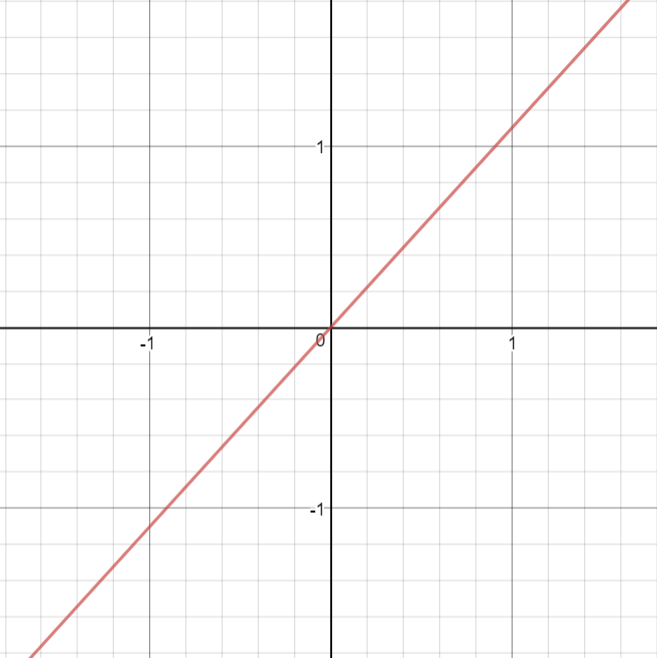
\includegraphics[width=0.9\linewidth]{fig/actfunc_linear.png}
                  \caption{%
                      \begin{equation}
                          \begin{split}R(z,m) =
                              \begin{Bmatrix}
                                  z*m \\
                              \end{Bmatrix}
                          \end{split}
                      \end{equation}
                  }
                  \label{fig:actfunc_lin}
              \end{subfigure}%
              \begin{subfigure}{0.5\textwidth}
                  \centering
                  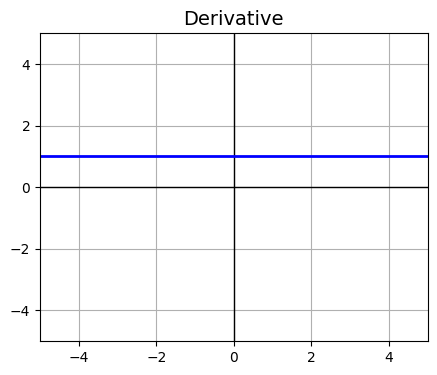
\includegraphics[width=0.9\linewidth]{fig/actfunc_linear_der.png}
                  \caption{%
                      \begin{equation}
                          \begin{split}R'(z,m) =
                              \begin{Bmatrix}
                                  m \\
                              \end{Bmatrix}
                          \end{split}
                      \end{equation}
                  }
                  \label{fig:actfunc_lin_der}
              \end{subfigure}
          \end{figure}
          ข้อดี:
          \begin{itemize}
              \item เป็น Activation แบบที่เป็นช่วง (Range) ซึ่งมีประสิทธิดีกว่าฟังก์ชันแบบไบนารี่
          \end{itemize}
          ข้อเสีย:
          \begin{itemize}
              \item อนุพันธ์ของฟังก์ชันนี้เป็นค่าคงที่ นั่นคือเกรเดียนต์ของฟังก์ชันนี้จึงไม่มีความสัมพันธ์กับอินพุต
          \end{itemize}

    \item \textbf{ELU} ย่อมาจาก Exponential Linear Unit เป็นฟังก์ชันที่พยายามทำให้ Cost นั้นลู่เข้าสู่ศูนย์และให้ประสิทธิภาพที่ดี%
          มากขึ้น โดยพารามิเตอร์ที่ควบคุมประสิทธิภาพของ ELU ก็คือ $\alpha$ ซึ่งควรจะต้องมีค่าเป็นบวกเสมอ
          \idxen{Activation Function!ELU}
          \begin{figure}[H]
              \centering
              \begin{subfigure}{0.5\textwidth}
                  \centering
                  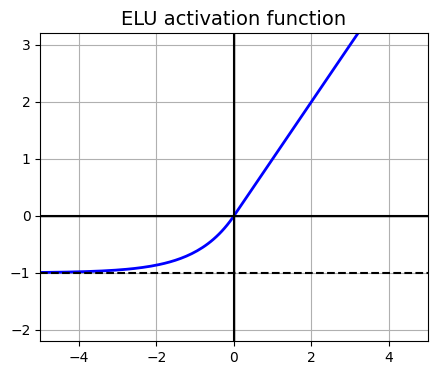
\includegraphics[width=0.9\linewidth]{fig/actfunc_elu.png}
                  \caption{%
                      \begin{equation}
                          \begin{split}R(z) =
                              \begin{Bmatrix}
                                  z                & z > 0  \\
                                  \alpha (e^z – 1) & z <= 0
                              \end{Bmatrix}
                          \end{split}
                      \end{equation}
                  }
                  \label{fig:actfunc_elu}
              \end{subfigure}%
              \begin{subfigure}{0.5\textwidth}
                  \centering
                  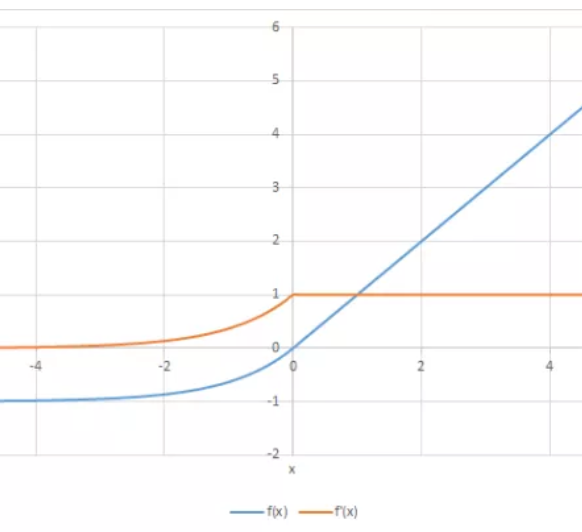
\includegraphics[width=0.9\linewidth]{fig/actfunc_elu_der.png}
                  \caption{%
                      \begin{equation}
                          \begin{split}R'(z) =
                              \begin{Bmatrix}
                                  1          & z>0 \\
                                  \alpha e^z & z<0
                              \end{Bmatrix}
                          \end{split}
                      \end{equation}
                  }
                  \label{fig:actfunc_elu_der}
              \end{subfigure}
          \end{figure}
          ข้อดี:
          \begin{itemize}
              \item ฟังก์ชัน ELU นั้นมีความราบเรียบ (Smooth) ยอ่างช้า ๆ จนกว่าค่าเอาต์พุตของฟังก์ชันจะมีค่าเท่ากับ $-\alpha$

              \item เราสามารถใช้ฟังก์ชัน ELU แทน ReLU ได้ในบางกรณีเพราะทั้งสองฟังก์ชันนี้มีความคล้ายกันมาก

              \item ELU สามารถให้เอาต์พุตที่มีค่าเป็นลบได้ แต่ว่าฟังก์ชัน ReLU นั้นให้เอาต์พุตที่เป็นบวกเสมอ
          \end{itemize}
          ข้อเสีย:
          \begin{itemize}
              \item สำหรับกรณีที่ $x > 0$ การใช้ฟังก์ชัน ELU อาจจะทำให้เกิดปัญหาได้ (เกิดการระเบิดหรือ Blow Up) จะทำให้เอาต์พุตอยู่ในช่วง
                    $[0,\infty)$
          \end{itemize}

    \item \textbf{ReLU}\autocite{glorot2011} ย่อมาจาก Rectified Linear Units เป็นฟังก์ชันกระตุ้นที่มีความสามารถในการ%
          เรียนรู้ฟังก์ชันหรือความสัมพันธ์ที่ไม่เป็นเชิงเส้นได้ดีมาก (ดีกว่าฟังก์ชัน Sigmoid)
          \idxen{Activation Function!ReLU}
          \begin{figure}[H]
              \centering
              \begin{subfigure}{0.5\textwidth}
                  \centering
                  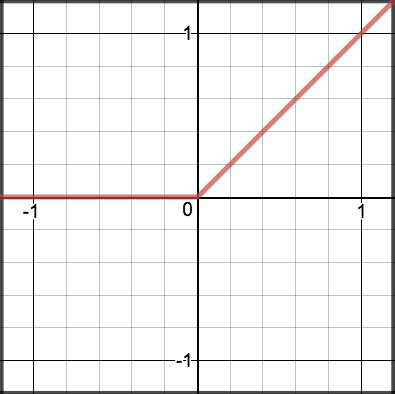
\includegraphics[width=0.9\linewidth]{fig/actfunc_relu.png}
                  \caption{%
                      \begin{equation}
                          \begin{split}R(z) =
                              \begin{Bmatrix}
                                  z & z > 0  \\
                                  0 & z <= 0
                              \end{Bmatrix}
                          \end{split}
                      \end{equation}
                  }
                  \label{fig:actfunc_relu}
              \end{subfigure}%
              \begin{subfigure}{0.5\textwidth}
                  \centering
                  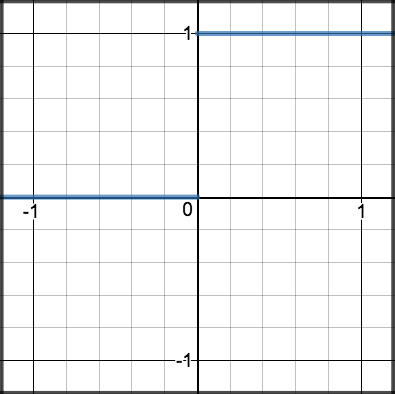
\includegraphics[width=0.9\linewidth]{fig/actfunc_relu_der.png}
                  \caption{%
                      \begin{equation}
                          \begin{split}R'(z) =
                              \begin{Bmatrix}
                                  1 & z>0 \\
                                  0 & z<0
                              \end{Bmatrix}
                          \end{split}
                      \end{equation}
                  }
                  \label{fig:actfunc_relu_der}
              \end{subfigure}
          \end{figure}

          ข้อดี:
          \begin{itemize}
              \item ReLU แก้ปัญหา Vanishing Gradient Problem ได้

              \item ฟังก์ชัน ReLU นั้นเรียบง่ายกว่า Sigmoid และ Tanh จึงทำให้การคำนวณของฟังก์ชัน ReLU นั้นเร็วกว่าและสิ้นเปลืองน้อยกว่า
          \end{itemize}
          ข้อเสีย:
          \begin{itemize}
              \item ควรใช้ฟังก์ชัน ReLU เฉพาะใน Hidden Layer ของ Neural Network เท่านั้น

              \item ในระหว่างการฝึกสอนโมเดลด้วย ReLU ของบางกรณีนั้น การคำนวณ Gradient อาจจะมีปัญหาได้

              \item สำหรับการ Activation ของฟังก์ชัน ReLU ในช่วงที่ิอินพุต $x < 0$ ค่า Gradient จะเท่ากับ 0 เพราะว่า Weights
                    นั้นจะไม่ถูกปรับค่าในระหว่างการทำ Gradient Descent

              \item เนื่องจากว่า ReLU นั้นมีความคล้ายกับ ELU ดังนั้นการใช้ฟังก์ชัน ReLU อาจจะทำให้เกิดปัญหาได้เพราะว่ามี Range คือ
                    $[0,\infty)$
          \end{itemize}

    \item \textbf{LeakyReLU}\autocite{he2015} เป็นฟังก์ชันที่ถุกพัฒนาต่อมาจาก ReLU ซึ่งได้มีการปรับปรุงให้มีประสิทธิภาพมากขึ้น%
          โดยทำการปรับค่าเอาต์พุต ในกรณีที่อินพุต $z < 0$ ค่าเอาต์พุตจะไม่เป็น 0 อีกต่อไป แต่จะเป็น $\alpha z$ แทน ซึ่งทำให้มีความ General
          มากกว่าฟังก์ชัน ReLU ซึ่งโดยปกติแล้วจะกำหนดให้ $\alpha = 0.01$
          \idxen{Activation Function!LeakyReLU}
          \begin{figure}[H]
              \centering
              \begin{subfigure}{0.5\textwidth}
                  \centering
                  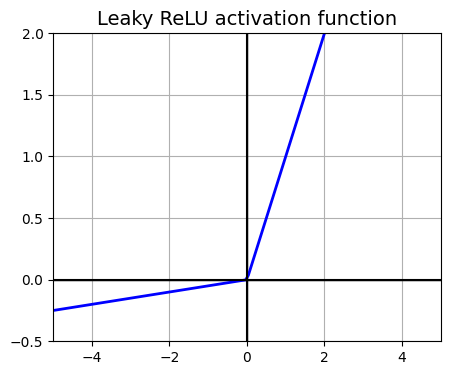
\includegraphics[width=0.9\linewidth]{fig/actfunc_leakyrelu.png}
                  \caption{%
                      \begin{equation}
                          \begin{split}R(z) =
                              \begin{Bmatrix}
                                  z        & z > 0  \\
                                  \alpha z & z <= 0
                              \end{Bmatrix}
                          \end{split}
                      \end{equation}
                  }
                  \label{fig:actfunc_leakyrelu}
              \end{subfigure}%
              \begin{subfigure}{0.5\textwidth}
                  \centering
                  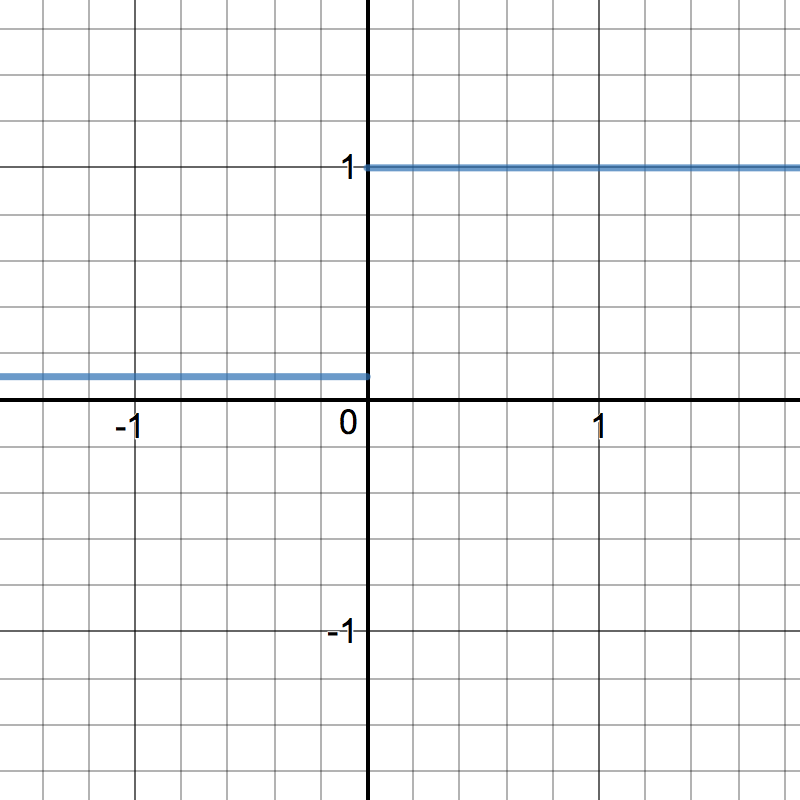
\includegraphics[width=0.9\linewidth]{fig/actfunc_leakyrelu_der.png}
                  \caption{%
                      \begin{equation}
                          \begin{split}R'(z) =
                              \begin{Bmatrix}
                                  1      & z>0 \\
                                  \alpha & z<0
                              \end{Bmatrix}
                          \end{split}
                      \end{equation}
                  }
                  \label{fig:actfunc_leakyrelu_der}
              \end{subfigure}
          \end{figure}

          ข้อดี:
          \begin{itemize}
              \item LeakyReLU สามารถแก้ปัญหาของ ReLU ได้โดยการทำให้มีเอาต์พุตเป็น Slope ที่มีความชันน้อย ๆ
          \end{itemize}
          ข้อเสีย:
          \begin{itemize}
              \item เนื่องจากว่า Range ของ LeakyReLU นั้นเป็นเส้นตรง ดังนั้นจึงไม่เหมาะที่จะนำฟังก์ชันนี้มาใช้กับปัญหา Classification
                    ที่ซับซ้อน ซึ่งในกรณีดังกล่าวการใช้ฟังก์ชัน Sigmoid หรือ Tanh จะเหมาะสมกว่า
          \end{itemize}

    \item \textbf{Sigmoid}\autocite{wilson1972} เป็นหนึ่งในฟังก์ชันกระตุ้นที่มีประสิทธิภาพสูงมากในการนำมาใช้กับ Neural Network
          โดยฟังก์ชันนี้ทำการนำค่าอินพุตมาคำนวณโดยใช้ฟังก์ชัน Exponential ซึ่งให้ค่าเอาต์พุตที่อยู่ระหว่าง $(0, 1)$ ดังนั้นจึงทำให้ฟังก์ชันนี้มี%
          คุณสมบัติหลายอย่างที่ฟังก์ชันกระตุ้นควรมี เช่น ความไม่เป็นเส้นตรง, มีความต่อเนื่อง, สามารถหาอนุพันธ์ได้ตลอดช่วง, มีความโมโนโทนิค
          (Monotonic) และมีเอาต์พุตที่อยู่ในช่วงที่แน่นอน
          \idxen{Activation Function!Sigmoid}
          \begin{figure}[H]
              \centering
              \begin{subfigure}{0.5\textwidth}
                  \centering
                  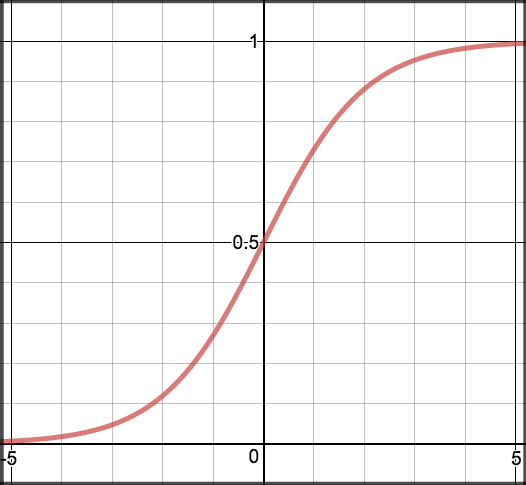
\includegraphics[width=0.9\linewidth]{fig/actfunc_sigmoid.png}
                  \caption{%
                      \begin{equation}
                          S(z) = \frac{1} {1 + e^{-z}}
                      \end{equation}
                  }
                  \label{fig:actfunc_sigmoid}
              \end{subfigure}%
              \begin{subfigure}{0.5\textwidth}
                  \centering
                  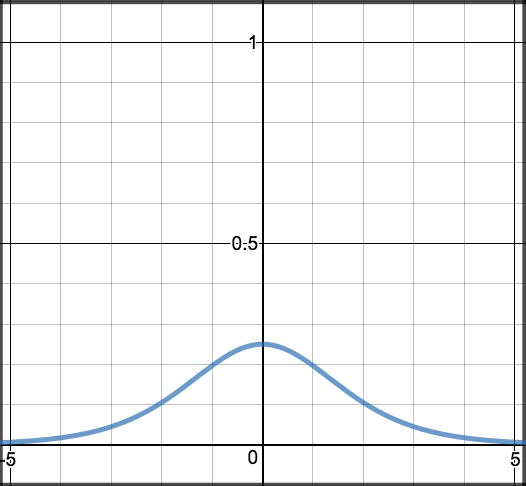
\includegraphics[width=0.9\linewidth]{fig/actfunc_sigmoid_der.png}
                  \caption{%
                      \begin{equation}
                          S'(z) = S(z) \cdot (1 - S(z))
                      \end{equation}
                  }
                  \label{fig:actfunc_sigmoid_der}
              \end{subfigure}
          \end{figure}

          ข้อดี:
          \begin{itemize}
              \item มีความไม่เป็นเส้นตรง

              \item ฟังก์ชัน Sigmoid มีอนุพันธืที่มีความราบเรียบ

              \item เหมาะสำหรับการนำไปใช้กับโจทย์ Classification

              \item ฟังก์ชัน Sigmoid มี Range คือ $(0,1)$ ซึ่งไม่เหมือนกับ Range ของฟังก์ขันเส้นตรงซึ่งมีค่าที่ไม่อยู่ในช่วงที่แน่นอนนั่นคือ
                    $-\infty, \infty$
          \end{itemize}
          ข้อเสีย:
          \begin{itemize}
              \item กรณีที่ค่าอินพุตมีค่ามาก ๆ ค่าเอาต์พุตของ Sigmoid จะมีการเปลี่ยนแปลงที่น้อยมาก ๆ

              \item ฟังก์ชัน Sigmoid ทำให้เกิดปัญหา Vanishing Gradient Problem ได้

              \item เอาต์พุตของฟังก์ชัน Sigmoid มีจุดกึ่งกลางที่ไม่ใช่ 0 (Not Zero-centered) ทำให้การเปลี่ยนแปลงของ Gradient
                    นั้นมีค่าที่อยู่ห่างจากฟังก์ชันเดิมมาก ๆ ซึ่งเป็นสาเหตุที่ทำให้การ Optimization นั้นยากขึ้น

              \item ในบางกรณีนั้นการใช้ฟังก์ชัน Sigmoid จะทำให้การเรียนรู้ของ Neural Network นั้นทำได้ยากและช้า
          \end{itemize}

    \item \textbf{Tanh} เป็นฟังก์ชันกระตุ้นแบบไม่เป็นเชิงเส้นที่มี Range อยู่ระหว่าง -1 ถึง 1 $(-1, 1)$ สิ่งที่ฟังก์ชัน Tanh ต่างจาก%
          ฟังก์ชัน Sigmoid ก็คือเอาต์พุตมีจุดกึ่งกลางอยู่ที่ 0 (Zero-centered) จึงทำให้ฟังก์ชันนี้ได้รับความนิยมมากกว่า Sigmoid นั่นเอง
          \idxen{Activation Function!Tanh}
          \begin{figure}[H]
              \centering
              \begin{subfigure}{0.5\textwidth}
                  \centering
                  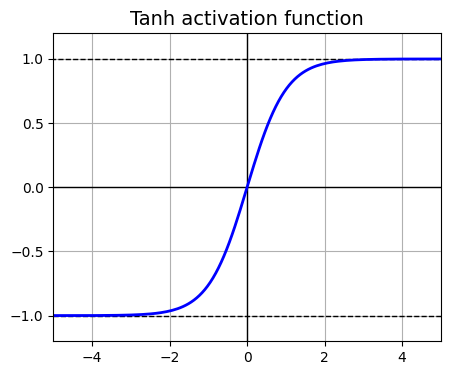
\includegraphics[width=0.9\linewidth]{fig/actfunc_tanh.png}
                  \caption{%
                      \begin{equation}
                          tanh(z) = \frac{e^{z} - e^{-z}}{e^{z} + e^{-z}}
                      \end{equation}
                  }
                  \label{fig:actfunc_tanh}
              \end{subfigure}%
              \begin{subfigure}{0.5\textwidth}
                  \centering
                  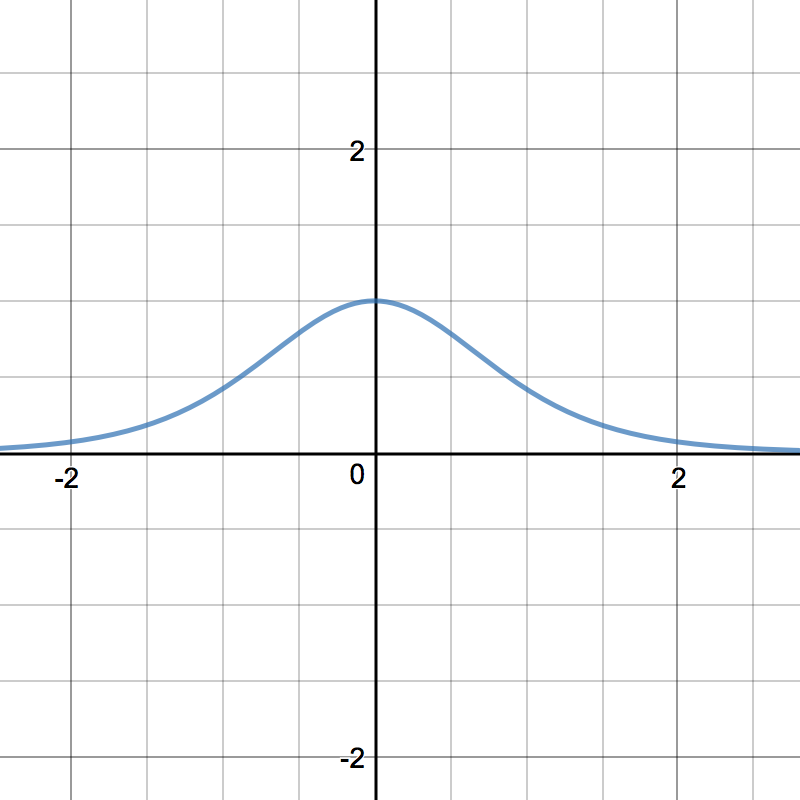
\includegraphics[width=0.9\linewidth]{fig/actfunc_tanh_der.png}
                  \caption{%
                      \begin{equation}
                          tanh'(z) = 1 - tanh(z)^{2}
                      \end{equation}
                  }
                  \label{fig:actfunc_tanh_der}
              \end{subfigure}
          \end{figure}

          ข้อดี:
          \begin{itemize}
              \item Gradient ของฟังก์ชัน Tanh มีค่าการเปลี่ยนแปลงของ Slope ที่ดีกว่า Gradient ของฟังก์ชัน Sigmoid
          \end{itemize}
          ข้อเสีย:
          \begin{itemize}
              \item ฟังก์ชัน Tanh ยังคงมีปัญหาเกี่ยวกับ Vanishing Gradient Problem
          \end{itemize}

    \item \textbf{Softmax} เป็นฟังก์ชันกระตุ้นที่คำนวณ Probability Distribution ของเหตุการณ์ทั้งหมด $n$ เหตุการณ์ที่แตกต่างกัน
          กล่าวง่าย ๆ คือฟังก์ชันนี้ทำการคำนวณคลาส (Class) ของเป้าหมายของเราให้อยู่ในรูปของค่าความน่าจะเป็นซึ่งจะถูกนำมาใช้ในการกำหนด%
          หรือทำนายคลาสของเหตุการณ์ที่เราสนใจ
          \idxen{Activation Function!Softmax}
          \begin{equation}
              \sigma(z_i) = \frac{e^{z_{i}}}{\sum_{j=1}^K e^{z_{j}}} \ \ \ for\ i=1,2,\dots,K
          \end{equation}
\end{itemize}

ถ้าหากผู้อ่านต้องการศึกษาการเขียนโค้ดสำหรับพล็อตกราฟฟังก์ชันกระตุ้นแบบต่าง ๆ สามารถดูได้ที่
\url{https://github.com/siebenrock/activation-functions}

%--------------------------
\section{ฟังก์ชันสูญเสีย}
\label{sec:loss_func}
\idxboth{ฟังก์ชันสูญเสีย}{Loss Function}
\idxboth{ฟังก์ชันต้นทุน}{Cost Function}
\idxboth{ฟังก์ชันความคลาดเคลื่อน}{Error Function}
%--------------------------

%--------------------------
\subsection{ความสำคัญของฟังก์ชันสูญเสีย}
\label{ssec:why_loss_func}
%--------------------------

ฟังก์ชันสูญเสีย (Loss Function หรือ Cost Function) เป็นฟังก์ชันความคลาดเคลื่อน (Error Function) รูปแบบหนึ่งซึ่งมีความสำคัญมากใน
Neural Network (จริง ๆ แล้วเราจะถือว่า Loss Function กับ Error Function นั้นเป็นสิ่งเดียวกันก็ได้) เพราะว่าเป็นฟังก์ชันคณิตศาสตร์ที่
Map ค่าเหตุการณ์ (Event) จากอินพุตหลาย ๆ ตัว ให้ออกมาเป็นค่า Error เพียงแค่เดียวซึ่งเป็นค่าที่ระบุถึง Cost ของเหตุการณ์นั้น ๆ โดย Loss
Function ถูกใช้ในการทำ Optimization นั่นก็คือการหาวิธีที่ทำให้ค่าเอาต์พุตของของ Loss Function นั้นมีค่าน้อยที่สุด เรียกว่า Minimization

\begin{figure}[H]
    \centering
    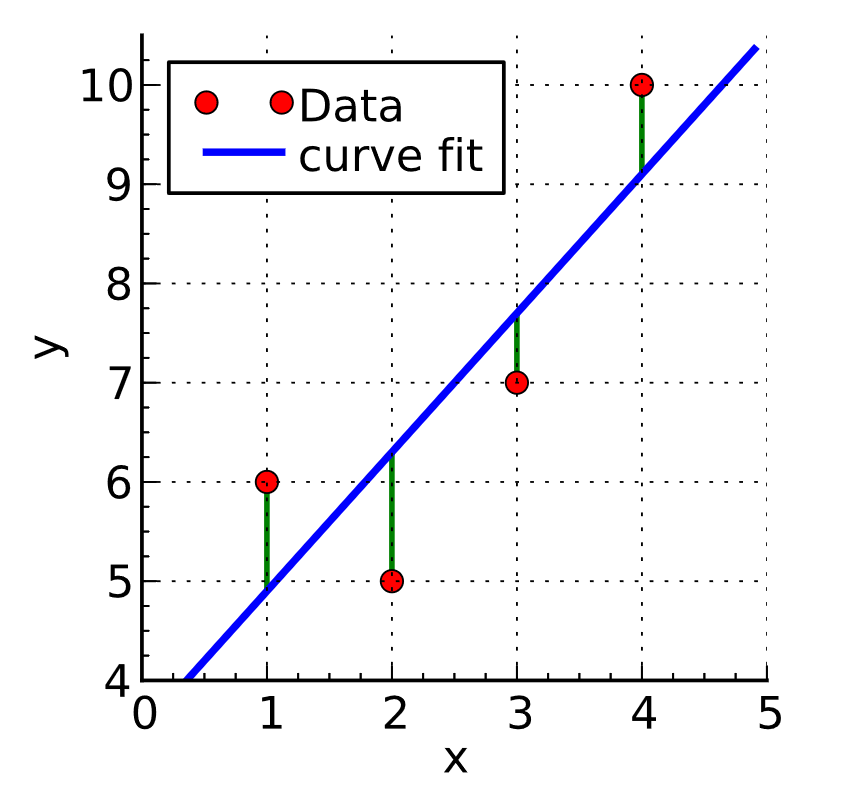
\includegraphics[width=0.7\linewidth]{fig/least-squares-fitting.png}
    \caption{แสดงการทำ Least Squares Fitting โดยมีพิกัดตำแหน่งของข้อมูลแต่ละตัว (จุดสีแดง) ดังนี้ $(1,6)$, $(2,5)$, $(3,7)$
        และ $(4,10)$ และเส้นตรงที่ได้จากการประมาณค่าด้วยวิธี Least Squares Estimation นั้น (เส้นสีน้ำเงิน) (เครดิตภาพ:
        \url{https://en.wikipedia.org/wiki/Linear_least_squares})}
    \label{fig:least_square_fitting}
\end{figure}

แนวคิดของ Loss Function ก็คือเราต้องการตัวชี้วัดที่เป็นตัวเลขค่าเดียวที่สามารถบอกได้ว่าโมเดล ML ที่ฝึกสอนมาแล้วนั้นทำงานได้ดีแค่ไหน
โดยถ้าหากดูจากภาพที่ \ref{fig:least_square_fitting} โดยเปรียบเทียบเอาต์พุตของโมเดลนั่นก็คือ $\hat{y}$ กับข้อมูลเอาต์พุตตัวอย่าง
$y$ นั่นก็คือจุดสีแดงและมีค่าเส้นน้ำเงินที่เป็นเส้นที่เกิดจากการ Fitting และมีเส้นสีเขียวที่บ่งบอกว่าจุดสีแดงแต่ละจุดนั้นมีการเบี่ยงเบน (Deviation)
ออกจากเส้นสีน้ำเงินมากน้อยเพียงใด

%--------------------------
\subsubsection{ฟังก์ชันสูญเสียสำหรับโจทย์ประเภท Regression}
\label{sssec:loss_func_reg}
%--------------------------

การทำ Regression นั้นจะเกี่ยวข้องกับการทำนายค่าที่แน่นอนและมีความต่อเนื่อง ดังนั้น Loss Function ที่เหามะสมจึงจะต้องสามารถที่จะอธิบาย%
ความต่อเนื่องของเอาต์พุตของแต่ละจุดในชุดข้อมูลได้ด้วย ตัวอย่างของ Loss Function ที่นิยมใช้ในโจทย์ประเภท Regression ของชุดข้อมูลที่มี
$n$ จำนวนข้อมูลและมีค่าเอาต์พุตที่ได้จากการทำนายที่เป็น $\hat{y}$ และคำตอบอ้างอิง (Reference หรือ Label) คือ $y$ มีดังต่อไปนี้

\begin{equation}\label{eq:mae}
    \text{MAE} = \frac{1}{n} \sum_{i=1}^{n} | y_{i} - \hat{y}_{i} |
\end{equation}
\idxen{Error Function!MAE}

\begin{equation}\label{eq:mape}
    \text{MAPE} = \frac{1}{n} \sum_{i=1}^{n} \left| \frac{y_{i} - \hat{y}_{i}}{x_{i}} \right| \times 100
\end{equation}
\idxen{Error Function!MAPE}

\begin{equation}\label{eq:mse}
    \text{MSE} = \frac{1}{n} \sum_{i=1}^{n} \left( y_{i} - \hat{y}_{i} \right)^2
\end{equation}
\idxen{Error Function!MSE}

\begin{equation}\label{eq:maxae}
    \text{MaxAE} = \max\{y_{i} - \hat{y}_{i}\}, i = 1, 2, ..., n
\end{equation}
\idxen{Error Function!MaxAE}

\begin{equation}\label{eq:maxape}
    \text{MaxAPE} = \max\left\{\left| \frac{y_{i} - \hat{y}_{i}}{x_{i}} \right| \times 100 \right\}, i = 1, 2,
    ..., n
\end{equation}
\idxen{Error Function!MaxAPE}

\begin{equation}\label{eq:rmsd}
    \text{RMSD} = \sqrt{ \frac{1}{n} \sum_{i=1}^{n} (y_{i} - \hat{y}_{i})^{2} }
\end{equation}
\idxen{Error Function!RMSD}

\begin{equation}\label{eq:grmsd}
    \text{GRMSD} = \sqrt[2n]{ \prod_{i=1}^{n} (y_{i} - \hat{y}_{i})^{2} }
\end{equation}
\idxen{Error Function!GRMSD}

\begin{equation}\label{eq:gwrmsd}
    \text{GWRMSD} = \sqrt{\frac{\sum_{i=1}^{n} \zeta_{i} (y_{i} - \hat{y}_{i})^{2}}{\sum_{i=1}^{n} \zeta_{i}}}
\end{equation}
\idxen{Error Function!GWRMSD}

\noindent โดยที่ $\zeta_{i} = e^{-(y_{i} - \hat{y}_{i}) / c}$

\begin{equation}\label{eq:huber}
    L_{\delta}=
    \left\{\begin{matrix}
        \frac{1}{2}(y - \hat{y})^{2}             & \text{if} \left | (y - \hat{y})  \right | < \delta \\
        \delta ((y - \hat{y}) - \frac1 2 \delta) & \text{otherwise}
    \end{matrix}\right.
\end{equation}
\idxen{Error Function!Huber}

สำหรับ Loss Function ที่ \eqref{eq:mae} - \eqref{eq:gwrmsd} จะมีความคล้ายคลึงกัน แต่จะต่างกันตรงที่การปรับรูปแบบให้ฟังก์ชันที่เป็นความ%
แตกต่างระหว่างค่าอ้างอิงและค่าทำนายนั้นมีความไว (Sensitivity) ต่อ Outlier ที่ต่างกันไป สำหรับสมการที่ \eqref{eq:huber} นั้นคือ Huber
Loss ซึ่งจะมีความไวต่อค่าที่ห่างค่าผิดปกติ (Outlier)\footnote{ค่าผิดปกติหรือ Outlier คือค่าที่อยู่ห่างจากค่าส่วนใหญ่ในชุดข้อมูลมากเกินไป}
ที่น้อยกว่ากรณีของ MSE (สมการที่ \eqref{eq:mse}) เพราะว่าใน MSE เทอม $y_{i} - \hat{y}_{i}$ ถูกกำลังสองอยู่นั่นเอง

\noindent เพิ่มเติม: MAE กับ MSE นั้นจะมีชื่อเรียกอีกอย่างว่า L1 และ L2 ด้วย

%--------------------------
\subsubsection{ฟังก์ชันสูญเสียสำหรับโจทย์ประเภท Classification}
\label{sssec:loss_func_class}
%--------------------------

Loss Function สำหรับโจทย์แบบ Classfication นั้นจะแตกต่างจาก Regression โดยสิ้นเชิงเนื่องจากว่าเราไม่ได้ทำการหาค่าระยะห่างระหว่าง%
จุดข้อมูลที่ได้จากการทำนายแล้ว แต่จะเป็นการหาความน่าจะเกิดที่เกิดขึ้นระหว่างข้อมู,ที่มีความไม่ต่อเนื่องกัน (Discrete Class Output) ซึ่งจะ%
ออกจากกันโดยสิ้นเชิง กล่าวคือโจทย์ประเภทนี้จะเป็นการแบ่งชุดข้อมูลออกเป็นคลาสหลาย ๆ คลาสที่แตกต่างกันโดยขึ้นอยู่กับพารามิเตอร์ที่ต่างกัน
ซึ่งหน้าที่ของ Loss Function สำหรับโจทย์ประเภทนี้คือจะต้องทำการคำนวณความน่าจะเป็นว่าควรจะต้องเพิ่มหรือระบุว่าข้อมูลใหม่นั้นควรจะต้องถูก%
จัดเข้าไปอยู่ในกลุ่มไหน

\noindent $\bullet$ Cross-entropy คือการวัดความแตกต่างระหว่างการกระจายตัวของความน่าจะเป็น 2 กลุ่มของตัวแปรแบบสุ่มของเหตุการณ์%
ที่เราสนใจ (กลุ่มหรือ Class ในชุดข้อมูล) โดยกรณีที่มีแค่ 2 Class $(M = 2)$ เรามีชื่อเรียกฟังก์ชันประเภทนี้ว่า Binary Cross-entropy
และกรณีที่มีมากกว่า 2 Class $(M > 2)$ เราจะเรียกว่า Multiclass Cross-entropy หรือจะเรียกว่า Categorical Cross-entropy ก็ได้
ซึ่งทั้งสองแบบมีสมการดังต่อไปนี้

\begin{equation}\label{eq:binary_entro}
    H(p) = -{(y\log(p) + (1 - y)\log(1 - p))}
\end{equation}

\begin{equation}\label{eq:multiclass_entro}
    H(p) = -\sum_{c=1}^My_{o,c}\log(p_{o,c})
\end{equation}

\noindent โดยที่ $p$ คือความน่าจะเป็นของการสังเกต $o$ ใน Class $c$ และ $y$ คือตัวระบุ Class (เช่น 0 กับ 1) โดยที่ Binary
Cross-entropy นี้เป็น Loss Function ที่ได้รับความนิยมมากที่สุดสำหรับโจทย์ Classification ที่มีสองคลาส ซึ่งคำว่า Entropy นี้ก็หมายถึง%
เป็นการวัดความไม่แน่นอนของการสุ่ม (Randomness) ที่เกิดขึ้นในข้อมูลในขณะที่ถูก Process อยู่นั่นเอง และ Cross Entropy ก็คือการวัดความ%
แตกต่างของ Randomness ระหว่างตัวแปรสุ่มสองตัว

\noindent $\bullet$ Negative Log-likelihood (NLL)

\begin{equation}\label{eq:neg_log_like}
    l(y) = -{\log(p(y))}
\end{equation}

\noindent $\bullet$ Hinge Loss

\begin{equation}\label{eq:hinge_loss}
    l(y) = \max(0, 1 - y \cdot \hat{y})
\end{equation}

\noindent Hinge Loss เป็น Loss Function ที่ถูกพัฒนาขึ้นมาเพื่อใช้งานกับ Support Vector Machine โดยเฉพาะสำหรับการคำนวณระยะ%
ห่างที่มากที่สุด (Maximum Margin) จาก Hyperplane ถึง Class

\noindent $\bullet$ Kullback-Leibler (KL) Divergence

\begin{equation}\label{eq:kl_diver}
    KL(\hat{y} || y) = \sum_{c=1}^{M}\hat{y}_c \log \bigg( {\frac{\hat{y}_c}{y_c}} \bigg)
\end{equation}

\noindent เป็นการวัดว่าข้อมูลนั้นมีการกระจายตัวห่างไปจากค่าการกระจายตัวอ้างอิงมากน้อยแค่ไหน

\noindent $\bullet$ Jensen-Shannon (JS) Divergence

\begin{equation}\label{eq:jensen_shannon_diver}
    JS(\hat{y} || y) = \frac{1}{2} \left ( KL \left ( y||\frac{y+\hat{y}}{2} \right ) +
    KL \left ( \hat{y}||\frac{y+\hat{y}}{2} \right ) \right )
\end{equation}

%--------------------------
\subsection{คณิตศาสตร์ของฟังก์ชันสูญเสีย}
%--------------------------

ลำดับต่อมาเรามาดูกันที่คณิตศาสตร์ที่อยู่เบื้องหลังของ Loss Function กันครับ โดยจะมาดูว่าเราสามารถทำการปรับค่าพารามิเตอร์ต่าง ๆ ใน Neural
Network เช่น Weight ได้อย่างไร โดยผู้เขียนจะใช้ตัวอย่างโจทย์ Regression สองแบบนั่นคือ Linear Regression และ Logistic Regression

%--------------------------
\subsubsection{Linear Regression}
\idxen{Loss Function!Linear Regression}
%--------------------------

เราเริ่มต้นด้วยการกำหนดฟังก์ชันหลักสำหรับการทำ Linear Regression ดังนี้

\fbox{%
    \begin{minipage}{0.9\linewidth}
        \begin{align*}
             & \text{Linear Equation}:     &  & z = Xw + b                               \\[1.5ex]
             & \text{Activation Function}: &  & \text{None}                              \\[1.5ex]
             & \text{Prediction}:          &  & \hat{y} = z                              \\[0.5ex]
             & \text{Loss Function}:       &  & \mathcal{L} = \frac{1}{2}(\hat{y} - y)^2 \\[0.3ex]
        \end{align*}
    \end{minipage}}

เราสามารถเขียนโค้ดของฟังก์ชันด้วยภาษา Python ได้ดังนี้

\begin{lstlisting}[style=MyPython]
import numpy as np

weights = np.random.normal(size = n_features).reshape(n_features, 1)
bias = 0

def linear_regression_inference(inputs):
    return np.matmul(inputs, weights) + bias   

def calculate_error(x, y):
    # Mean Squared Error (Ignore taking an average)
    y_hat = linear_regression_inference(x)
    return 0.5 * (yhat - y)**2 
\end{lstlisting}

\vspace{1em}
นอกจากนี้เรายังสามารถคำนวณอนุพันธ์ (Derivative) ของ Loss Function เทียบกับ $z$ โดยใช้กฎลูกโซ่ได้ดังนี้

\begin{equation}\label{eq:loss_chain_rule}
    \frac{\partial \mathcal{L}}{\partial z} =
    \frac{\partial \mathcal{L}}{\partial \hat{y}} \frac{\partial \hat{y}}{\partial z}
\end{equation}

\noindent เริ่มต้นด้วยการหาอนุพันธ์ย่อยของ Loss Function เทียบกับค่า Prediction

\begin{equation}\label{eq:der_loss_pred}
    \frac{\partial \mathcal{L}}{\partial \hat{y}} = \hat{y} - y
\end{equation}

\noindent ขั้นตอนต่อมาคือเราหาอนุพันธ์ย่อยของ Prediction เทียบกับ Linear Equation แต่เนื่องจากว่า Linear Equation จริง ๆ แล้ว%
ก็คือ Prediction นั่่นเอง จึงทำให้อนุพันธ์ย่อยนั้นมีค่าเท่ากับ 1

\begin{equation}\label{eq:der_pred_lin_eq}
    \frac{\partial \hat{y}}{\partial z} = 1
\end{equation}

\noindent เมื่อเราทำการคูณสมการที่ \eqref{eq:der_loss_pred} กับ \eqref{eq:der_loss_pred} เข้าด้วยกัน เราจะได้อนุพันธ์ของ Loss
Function ตามที่ต้องการ

\begin{equation}\label{eq:der_loss_lin_eq}
    \frac{\partial \mathcal{L}}{\partial z} = \hat{y} - y
\end{equation}

\noindent จากตัวอย่างข้างต้นนี้ผู้อ่านจะพบว่า Linear Regression นั้นง่ายมาก แต่ตัวอย่างต่อไปจะมีความซับซ้อนมากขึ้นครับ

%--------------------------
\subsubsection{Logistic Regression}
\idxen{Loss Function!Logistic Regression}
%--------------------------

ตัวอย่างที่สองคือกรณีของ Logistic Regression โดยเรากำหนดฟังก์ชันต่าง ๆ ดังนี้

\fbox{%
    \begin{minipage}{0.9\linewidth}
        \begin{align*}
             & \text{Linear Equation}:     &  & z = Xw + b                                           \\[0.5ex]
             & \text{Activation Function}: &  & \sigma(z) = \frac{1}{1 + e^{-z}}                     \\[0.5ex]
             & \text{Prediction}:          &  & \hat{y} = \sigma(z)                                  \\[1.5ex]
             & \text{Loss Function}:       &  & \mathcal{L} = -(y\log\hat{y} + (1-y)\log(1-\hat{y})) \\[0.5ex]
        \end{align*}
    \end{minipage}}

\vspace{1em}
\noindent และเขียนโค้ดของฟังก์ชันได้ดังนี้\footnote{โดยทั่วไปแล้วในการคำนวณหา Error ของ Logistic Regression ควรจะทำการใส่%
    ค่าคงที่เข้าไปในฟังก์ชัน Log เพื่อป้องกันไม่ให้อินพุตของ Log นั้นเป็น 0}

\begin{lstlisting}[style=MyPython]
import numpy as np

weights = np.random.normal(size = n_features).reshape(n_features, 1)
bias = 0

def sigmoid(x):
    return 1 / (1 + np.exp(-x))

def logistic_regression_inference(x):
    return sigmoid(np.matmul(x, weights) + bias)

def calculate_error(x, y):
    # Binary Cross-Entropy
    y_hat = logistic_regression_inference(x)
    return -(y * np.log(y_hat) + (1 - y) * np.log(1 - y_hat))
\end{lstlisting}

\vspace{1em}
เราเริ่มต้นด้วยวิธีเดียวกันกับที่เราใช้ในตัวอย่างที่แล้วคือการใช้กฎลูกโซ่ (สมการที่ \eqref{eq:loss_chain_rule}) แล้วทำการหาอนุพันธ์ของแต่ละเทอม
ดังนี้

\begin{equation}
    \frac{\partial \mathcal{L}}{\partial \hat{y}} = -\frac{y}{\hat{y}} + \frac{1-y}{1-\hat{y}}
\end{equation}

ลำดับต่อไปก็คือการทำอนุพันธ์ย่อยของ Prediction เทียบกับฟังก์ชัน $z$ ซึ่งสามารถทำได้ดังนี้

\begin{align*}
    \frac{\partial \hat{y}}{\partial z} & = \frac{\partial}{\partial z}\left[\frac{1}{1 + e^{-z}}\right] \\[0.75ex]
                                        & = \frac{e^{-z}}{(1 + e^{-z})^2}                                \\[0.75ex]
                                        & = \frac{1 + e^{-z} - 1}{(1 + e^{-z})^2}                        \\[0.75ex]
                                        & = \frac{1 + e^{-z}}{(1 + e^{-z})^2} - \frac{1}{(1 + e^{-z})^2} \\[0.75ex]
                                        & = \frac{1}{1 + e^{-z}} - \frac{1}{(1 + e^{-z})^2}              \\[0.75ex]
                                        & = \frac{1}{1 + e^{-z}} \left(1 - \frac{1}{1 + e^{-z}}\right)   \\[0.75ex]
                                        & = \hat{y}(1 - \hat{y}) \numberthis
\end{align*}

\noindent เมื่อเรามาถึงขั้นตอนนี้แล้ว ขั้นตอนต่อไปคือการรวมสมการอนุพันธ์ย่อยทั้งสองสมการเข้าด้วยกัน โดยสามารถทำได้ดังนี้

\begin{align*}\label{eq:der_loss_logis_eq}
    \frac{\partial \mathcal{L}}{\partial z} & = \left(-\frac{y}{\hat{y}} + \frac{1-y}{1-\hat{y}}\right)\hat{y}
    (1 - \hat{y})                                                                                                                  \\[0.75ex]
                                            & = -\frac{y}{\hat{y}}\hat{y}(1 - \hat{y}) + \frac{1-y}{1-\hat{y}}\hat{y}(1 - \hat{y}) \\[0.75ex]
                                            & = -y(1 - \hat{y}) + (1-y)\hat{y}                                                     \\[0.75ex]
                                            & = -y + y\hat{y} + \hat{y} - y\hat{y}                                                 \\[0.75ex]
                                            & = \hat{y} - y \numberthis
\end{align*}

\noindent ซึ่งเราจะพบว่าคำตอบของสมการที่ \eqref{eq:der_loss_lin_eq} และ \eqref{eq:der_loss_logis_eq} นั้นเท่ากันเลย

%--------------------------
\section{ตัวประเมินโมเดล}
\label{sec:metrics}
\idxboth{ตัวประเมินโมเดล}{Metrics}
%--------------------------

สิ่งที่เราใช้ในการประเมินหรือวัดประสิทธิภาพของโมเดลก็คือ Metric ซึ่ง Metric สำหรับโจทย์ประเภท Regression นั้นเราสามารถใช้ฟังก์ชัน%
ที่เป็น Loss Function ได้เลย (หัวข้อที่ \ref{sssec:loss_func_reg}) โดยด้านล่างคือตัวอย่างของโค้ดสำหรับการใช้ Metric

\begin{lstlisting}[style=MyPython]
from tensorflow.keras import metrics

model.compile(loss='mse', optimizer='adam',
              metrics=[metrics.mean_squared_error,
                       metrics.mean_absolute_error,
                       metrics.mean_absolute_percentage_error])
                       metrics.categorical_accuracy])
\end{lstlisting}

\vspace{1em}

แต่กรณีโจทย์ประเภท Classification นั้นเราจะต้องใช้ฟังก์ชันที่ต่างกันออกไป ฟังก์ชันต่อไปนี้คือ Metrics ที่มักจะถูกใช้สำหรับ Classification

\noindent $\bullet$ ประเภทวัดความถูกต้องและแม่นยำ

\begin{equation}
    \text{Accuracy} = \frac{TP+TN}{TP+TN+FP+FN}
\end{equation}

\begin{equation}
    \text{Precision} = \frac{TP}{TP+FP}
\end{equation}

\begin{equation}
    \text{Recall} = \frac{TP}{TP+FN}
\end{equation}

\begin{align}
    \text{F1} & = \frac{2*Precision*Recall}{Precision+Recall} \nonumber \\
              & = \frac{2*TP}{2*TP+FP+FN}
\end{align}

\noindent $\bullet$ ประเภทวัดความว่องไวและความจำเพาะเจาะจง

\begin{equation}
    \text{Sensitivity} = \text{Recall} = \frac{TP}{TP+FN}
\end{equation}

\begin{equation}
    \text{Sensitivity} = \frac{TN}{FP+TN}
\end{equation}

นอกจากนี้ยังมี Area Under the Curve (AUC) ซึ่งเป็นการใช้พื้นที่ใต้เส้นโค้งสำหรับการแบ่งกลุ่ม (Classifier) อีกด้วย ผู้อ่านที่ต้องการศึกษา
Metrics เพิ่มเติมสามารถดูได้ที่ \url{https://neptune.ai/blog/keras-metrics}

%--------------------------
\section{ตัวปรับความเหมาะสม}
\label{sec:optimizer}
\idxboth{ตัวปรับความเหมาะสม}{Optimizer}
\idxboth{การปรับความเหมาะสม}{Optimization}
%--------------------------

ตัวปรับความเหมาะสมหรือปรับประสิทธิภาพการเรียนรู้ของโมเดล (Optimizer) เป็นฟังก์ชันทางคณิตศาสตร์ซึ่งขึ้นอยู่กับพารามิเตอร์ที่เรียนรู้ได้ของโมเดล
เช่น Weight และ Bias ซึ่ง Optimizer เป็นสิ่งที่จะช่วยให้โมเดลทราบวิธีการเปลี่ยน Weight และ Learning Rate ของ Neural Network
เพื่อลดค่า Loss หรือ Error ที่เกิดขึ้นให้น้อยลงในแต่ละรอบของการฝึกสอนโมเดล

\noindent ตัวอย่างของ Optimizer ที่ได้รับความนิยมและมีประสิทธิภาพที่ยอดเยี่ยม

\noindent $\bullet$ Stochastic Gradient Descent (SGD) เป็นฟังก์ชันที่อัพเดทค่าพารามิเตอร์ในทุก ๆ ชุดข้อมูลที่ใช้ในการฝึกฝน SGD
เป็นอัลกอริทึมที่ค่อนข้างไว โดยอัพเดทแค่ครั้งเดียวต่อการฝึกสอนโมเดล 1 รอบ นอกจากนี้ยังมีสิ่งที่เรียกว่าโมเมนตัม (Momentum) ซึ่งถูกพัฒนา%
ขึ้นมาเพื่อเร่งความเร็วในการ Opitmization ของ SGD โดยจะเป็นตัวที่เข้ามาแก้ปัญหาความแปรปรวนที่เกิดขึ้นใน SGD ซึ่งทำให้เกิดความยากในการ%
ที่จะลู่เข้าจุดที่ต่ำที่สุดได้ โดยการให้ความสำคัญในการพุ่งไปยังทิศทางที่ใกล้จุดกลางมากที่สุดก่อนแล้วทำให้ทิศทางที่ไม่เกี่ยวข้องความสำคัญลดลง
โดยสามารถอ่านรายละเอียดเพิ่มเติมได้ในหัวข้อที่ \ref{ssec:stochastic_grad}
\idxen{Gradient Descent!Stochastic}
\idxen{Optimizer!Stochastic Gradient Descent}

\noindent $\bullet$ Mini-batch Stochastic Gradient Descent ถูกพัฒนาขึ้นเพื่อแก้ปัญหาของ Gradient Descent (GD)
โดยการนำข้อดีของ GD แบบธรรมดาและ SGD มารวมกัน โดยสำหรับอัลกอริทึมนี้จะทำการอัพเดทค่าเป็น \enquote{ชุด} โดยภายในแต่ละชุดจะ%
ประกอบด้วยข้อมูลจำนวน $n$ ข้อมูล เราจึงเรียกเทคนิคนี้ว่าเป็น Mini-batch หรือจำนวนชุดข้อมูลขนาดเล็กนั่นเอง โดยสามารถอ่านรายละเอียด%
เพิ่มเติมได้ในหัวข้อที่ \ref{ssec:minibatch_grad}
\idxen{Gradient Descent!Mini-batch}
\idxen{Optimizer!Mini-batch Stochastic Gradient Descent}

\noindent $\bullet$ Adagrad เป็นฟังก์ชันที่สามารถปรับค่าอัตราเร็วในการเรียนรู้ (Learning Rate) ให้เหมาะสมกับพารามิเตอร์ได้
โดยจะมีการอัพเดทจำนวนมากสำหรับค่าพารามิเตอร์ที่มีจำนวนน้อย และอัพเดทน้อยถ้าค่าพารามิเตอร์มีจำนวนมากและด้วยเหตุนี้ Optimizer
ตัวนี้จึงเป็นที่นิยมสำหรับข้อมูลที่มีการกระจายตัว (Sparse Data)

\noindent $\bullet$ Adadelta เป็นฟังก์ชันที่พัฒนาต่อจาก AdaGrad โดยสามารถแก้ปัญหา Decaying Learning Rate ที่เกิดขึ้นใน
AdaGrad ได้ โดยเคล็ดลับก็คือแทนที่จะเก็บสะสมการคำนวณทั้งหมดที่ผ่านมาของ Gradient ใน AdaDelta นั้นจะถูกจำกัดการสะสมค่าการคำนวณของ
Gradient ได้เองเพื่อแก้ขนาดค่าของน้ำหนักที่จะเกิดขึ้น หมายความว่าแทนที่เราจะเก็บค่าน้ำหนักที่ได้รับการอัพเดทมาก่อนหน้านี้ที่ยังไม่เวิร์ค
เราจะเปลี่ยนเป็นการหาผลรวมของ Gradients แทน ซึ่งจะทำแบบนี้ซ้ำไปเรื่อย ๆ เพื่อการแก้ปัญหา Decaying Learning Rate ของ Gradients
ที่ผ่านมาทั้งหมด
\idxen{Optimizer!Adadelta}

\noindent $\bullet$ Adam ย่อมาจาก \enquote{Adaptive Moment Estimation} เป็นวิธีการสุ่มเกรเดียนต์ที่อิงจากการประมาณค่าแบบปรับตัว
(Adaptive Estimation) ของช่วงเวลาอันดับที่หนึ่งและอันดับสอง ซึ่งความสามารถของ Adam ก็คือสามารถปรับอัตราเร็วของการเรียนรู้พารามิเตอร์%
ในแต่ละครั้งได้และยังสามารถแก้ปัญหาการลดลงที่เร็วเกินไป (Decaying) ของ Gradients ในแต่ละ Step ที่ผ่านมาได้เหมือนกับ AdaDelta
อีกทั้งยังอธิบายการเกิด Decaying Average ของ Gradients ที่ผ่านมาได้อีกด้วย ซึ่งจะเหมือนกับโมเมนตัมนั่นเอง

Adam เป็นอัลกอริทึมเป็นที่นิยมมากที่สุดเพราะรวมข้อดีของแต่ละอัลกอริทึมที่อธิบายไว้ก่อนหน้านี้เข้าด้วยกัน และแก้ปัญหาหรือข้อบกพร่อมออกไป
เช่น Decaying Learning Rate ของ Adagrad และยังมีความเร็วที่มากกว่า GD และลดปัญหาการแกว่งของพารามิเตอร์ได้อีกด้วย
\idxen{Optimizer!Adam}

นอกเหนือจากตัวปรับความเหมาะสมข้างต้นแล้ว ยังมีอัลกอริทึมอีกหลายแบบที่ได้รับความนิยม เช่น Conjugate Gradients, Momentum (ใช้ใน
Stochastic Gradient Descent), Broyden-Fletcher-Goldfarb-Shanno (BFGS), Nesterov Momentum, วิธีของ Newton, และ
RMSProp ซึ่งผู้อ่านสามารถศึกษาเพิ่มเติมได้จากหนังสือ Algorithms for Optimization\autocite{kochenderfer2019} โดย Mykel J.
Kochenderfer โดยสามารถอ่านและดาวน์โหลดได้ฟรีที่ \url{https://algorithmsbook.com}

%--------------------------
\section{สถาปัตยกรรมของโครงข่ายประสาท}
\label{sec:arch_nn}
\idxboth{โครงข่ายประสาทเทียม!สถาปัตยกรรม}{Neural Network!Architecture}
%--------------------------

สถาปัตยกรรม (Architecture) ของ Neural Network เปรียบเสมือนเป็นการจำลองหรือเลียนแบบการเชื่อมโยงเซลล์ประสาทเทียมเข้าด้วยกัน%
เป็นโครงข่ายประสาทซึ่งสามารถเชื่อมโยงแบบใดก็ได้อย่างไม่มีขอบเขตจำกัด อย่างไรก็ตาม ในทางปฏิบัตินั้น เทคนิคการเรียนรู้ของ Neural Network
มักจะถูกออกแบบมาให้ใช้งานได้กับสถาปัตยกรรม Neural Network ที่มีลักษณะเฉพาะเท่านั้น

%--------------------------
\subsection{โครงข่ายประสาทมาตรฐาน}
\label{ssec:std_nn}
%--------------------------

\paragraph{Perceptron} เพอร์เซ็ปตรอนเป็น Neural Network แบบที่ง่ายที่สุด โดยมีเพียงแค่หน่วยการเรียนรู้ที่รับข้อมูลอินพุตและคืนค่า%
เอาต์พุตออกมา ซึ่ง Perceptron คือองค์ประกอบพื้นฐานของ Neural Network ทั้งหมด
\idxboth{โครงข่ายประสาทเทียม!สถาปัตยกรรม!เพอร์เซ็ปตรอน}{Neural Network!Architecture!Perceptron}

\paragraph{Multi-layer Perceptron Neural Network}
เป็นการนำ Perceptron หลาย ๆ อันมารวมกัน ได้เป็น Neural Network ที่มีหลายชั้น ถูกนำมาใช้สำหรับปัญหาที่มีความซับซ้อนได้ผลเป็นอย่างดี
โดยมีกระบวนการฝึกฝนเป็นแบบมีผู้สอน (Supervised ML) และใช้ขั้นตอนการส่งค่าย้อนกลับ (Backpropagation) สำหรับการฝึกฝนกระบวน%
การส่งค่าย้อนกลับ
\idxboth{โครงข่ายประสาทเทียม!สถาปัตยกรรม!โครงข่ายแบบหลายชั้น}{Neural Network!Architecture!Multi-layer Perceptron}

\paragraph{Residual Networks} หรือ ResNet เป็น Neural Network ที่ถูกพัฒนาขึ้นเพื่อแก้ปัญหา Vanishing Gradient ซึ่งมักเจอได้%
บ่อยใน Deep Neural Network ที่มี Hidden Layer หลายชั้น โดยไอเดียของ ResNet คือการนำ Weights จากชั้นตื้น (Shallow Layer)
มาใช้ในชั้นลึก (Deep Layer)
\idxen{Neural Network!Architecture!Residual Network}

%--------------------------
\subsection{โครงข่ายประสาทแบบวนซ้ำ}
\label{ssec:rnn}
%--------------------------

โครงข่ายประสาทแบบวนซ้ำ (Recurrent Neural Network หรือ RNN)\autocite{abiodun2018} เป็นสถาปัตกรรมที่ถูกออกแบบเพื่อเพิ่ม%
ความสามารถในการจดจำข้อมูลในอดีตที่ได้เรียนรู้ไปแล้ว ซึ่งในที่นี้คือข้อมูลของชั้นก่อนหน้า นั่นก็เพราะว่า Deep Neural Network แบบทั่วไปนั้น%
มักจะนำข้อมูลของชั้นในปัจจุบันมาใช้เท่านั้นและไม่ได้มีการนำข้อมูลที่เป็น Memory มาใช้ ดังนั้น RNN จึงเหมาะกับการฝึกสอนโมเดลเพื่อเรียนรู้ข้อมูล%
ที่มีลักษณะเป็นแบบลำดับ (Sequential) และต่อเนื่องเป็นชุด ๆ (Series)
\idxboth{โครงข่ายประสาทเทียม!สถาปัตยกรรม!แบบวนซ้ำ}{Neural Network!Architecture!Recurrent Neural Network}

นอกจากนี้ RNN ยังได้ถูกนำไปพัฒนาต่อให้มีประสิทธิภาพมากขึ้น โดยมีอีก 2 สถาปัตยกรรมย่อยที่ได้รับความนิยม คือ
%
\begin{itemize}[topsep=0pt,noitemsep]\setlength\itemsep{0.5em}
    \item Long Short-Term Memory (LSTM)\autocite{hochreiter1997a}
          \idxen{Neural Network!Architecture!Long Short-Term Memory}
    \item Echo State Network (ESN)\autocite{jaeger2004}
          \idxen{Neural Network!Architecture!Echo State Network}
\end{itemize}

%--------------------------
\subsection{โครงข่ายประสาทแบบคอนโวลูชัน}
\label{ssec:cnn}
\idxboth{โครงข่ายประสาทเทียม!สถาปัตยกรรม!แบบคอนโวลูชัน}{Neural Network!Architecture!Convolutional Neural Network}
%--------------------------

โครงข่ายประสาทแบบคอนโวลูชัน (Convolutional Neural Network หรือ CNN)\autocite{alzubaidi2021} เป็นโครงข่ายประสาทเทียม%
ที่ได้แรงบันดาลใจมาจากสิ่งมีชีวิต (Bio-inspired) โดยที่ CNN จะจำลองการมองเห็นของมนุษย์ที่มองพื้นที่เป็นที่ย่อย ๆ และนำพื้นที่ย่อย ๆ
เหล่านั้นมาผนวกหรือผสานกันเพื่อดูว่าสิ่งที่มองเห็นอยู่นั้นเป็นอะไรกันแน่

ไอเดียหลักของ CNN คือการใช้ Layer ชนิดพิเศษที่เรียกว่า Convolution Layer (ถ้าแปลเป็นภาษาไทยก็จะได้ความหมายว่า ชั้นที่เกิดการม้วน%
ขดกันหรือพับไปพับมา) ซึ่งทำหน้าที่สกัด (Extract) องค์ประกอบส่วนต่าง ๆ ของภาพออกมา เช่น เส้นขอบของวัตถุต่าง ๆ เพื่อให้โมเดลสามารถ%
เรียนรู้ลักษณะของภาพได้อย่างมีประสิทธิภาพและแม่นยำ CNN จะใช้ Convolution Layer มาประกอบกับ Layer ชนิดอื่น เช่น Pooling Layer
แล้วนำกลุ่ม Layer ดังกล่าวมาซ้อนต่อ ๆ กันโดยอาจเปลี่ยน Hyperparameter บางอย่าง เช่น ขนาดของ Filter Layer (ซึ่งเป็นส่วนหนึ่งของ
Convolution Layer) และจำนวนช่อง (Channel) ของ Layer โดยวิธีการนำส่วนต่าง ๆ มาประกอบเข้าด้วยกันนี้สามารถทำได้หลายแบบ เช่น
LeNet, GoogLeNet, AlexNet, VGG, ResNet, Network-in-network, SqueezeNet, Xception, MobileNets, Inception Network

%--------------------------
\section{การสร้างและฝึกสอนโมเดลด้วย TensorFlow}
\label{sec:train_tf}
\idxboth{โครงข่ายประสาทเทียม!การฝึกสอนโมเดล}{Neural Network!Training}
\idxen{TensorFlow}
%--------------------------

ในหัวข้อนี้จะเป็นการยกตัวอย่างประกอบโค้ดของการสร้างและฝึกสอนโมเดลในการทำนายค่าสภาพการละลายของโมเลกุล ซึ่งค่าสภาพการละลายหรือ
Solubility เป็นความสามารถของสสารในการละลายในน้ำ ยิ่งสสารมีค่าการละลายสูงหมายความว่าสสารนั้นยิ่งละลายในน้ำได้ดี โดยเราจะใช้ Module
Keras ซึ่งเป็นไลบรารี่ที่ถูกพัฒนาให้เป็น API หลักของ TensorFlow ในการสร้างโมเดล Neural Network ซึ่งตั้งแต่ TensorFlow ได้อัพเกรด
Framework ครั้งใหญ่จากเวอร์ชัน 1 มาเป็นเวอร์ชัน 2 ก็ได้รวบ Keras เข้ามาเป็นส่วนหนึ่งของ TensorFlow เลย ซึ่งสามารถเรียกใช้งาน Keras
ได้ง่าย ๆ ผ่าน \pyinline{tensorflow.keras}\footnote{ดูรายละเอียดการสร้างโมเดลแบบ Sequential ของ Keras ได้ที่
    \url{https://keras.io/guides/sequential_model}}

\begin{enumerate}
    \item ขั้นตอนแรกเราจะต้องทำการกำหนดรายละเอียดของ Neural Network

          \begin{lstlisting}[style=MyPython]
import numpy as np
import tensorflow as tf

# Our hidden layer
# We only need to define the output dimension - 32.
hidden_layer = tf.keras.layers.Dense(32, activation="tanh")
# Last layer - which we want to output one number
# the predicted solubility.
output_layer = tf.keras.layers.Dense(1)

# Now we put the layers into a sequential model
model = tf.keras.Sequential()
model.add(hidden_layer)
model.add(output_layer)
\end{lstlisting}

          \vspace{1em}

    \item ทำการทดสอบโดยเรียกใช้โมเดลเพื่อแสดงข้อมูลของสสารสามตัวแรกในชุดข้อมูล

          \begin{lstlisting}[style=MyPython]
# Try out our model on first few datapoints
model(soldata[feature_names].values[:3])

# Output
<tf.Tensor: shape=(3, 1), dtype=float32, numpy=
array([[ 0.18162721],
        [-0.416314  ],
        [-0.32956678]], dtype=float32)>
\end{lstlisting}

          \vspace{1em}

    \item คอมไพล์โมเดล

          \begin{lstlisting}[style=MyPython]
model.compile(optimizer="SGD", loss="mean_squared_error")
\end{lstlisting}

          \vspace{1em}

    \item ฝึกสอนโมเดล

          \begin{lstlisting}[style=MyPython]
model.fit(train_data, epochs=50)
\end{lstlisting}

          \vspace{1em}

    \item ทำนายค่าความสามารถในการละลายของโมเลกุล

          \begin{lstlisting}[style=MyPython]
yhat = np.squeeze(model.predict(test_data))
test_y = soldata["Solubility"].values[:test_N]
\end{lstlisting}

          \vspace{1em}

    \item พล็อตกราฟเปรียบเทียบค่าสภาพการละลายที่ได้จากการทำนายและค่าอ้างอิง

          \begin{lstlisting}[style=MyPython]
plt.plot(test_y, yhat, ".")
plt.plot(test_y, test_y, "-")
plt.xlabel("Measured Solubility $y$")
plt.ylabel("Predicted Solubility $\hat{y}$")
plt.text(
    min(test_y) + 1,
    max(test_y) - 2,
    f"correlation = {np.corrcoef(test_y, yhat)[0,1]:.3f}",
)
plt.text(
    min(test_y) + 1,
    max(test_y) - 3,
    f"loss = {np.sqrt(np.mean((test_y - yhat)**2)):.3f}",
)
plt.show()
\end{lstlisting}

          \vspace{1em}
          \noindent ได้กราฟดังต่อไปนี้

          \begin{figure}[H]
              \centering
              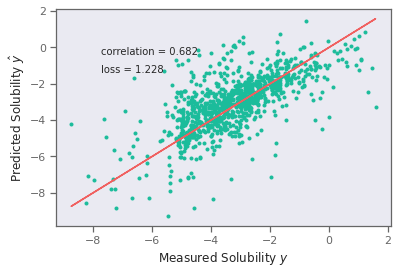
\includegraphics[width=0.8\linewidth]{fig/predict_solubility.png}
              \caption{เปรียบเทียบค่าสภาพการละลายที่ได้จากการทำนายและค่าอ้างอิง}
              \label{fig:pred_solubility}
          \end{figure}

          โดยภาพที่ \ref{fig:pred_solubility} แสดงการเปรียบเทียบค่าสภาพการละลายที่ได้จากการทำนายด้วย Neural Network และค่าอ้างอิง
          เส้นตรงสีแดงที่ลากผ่านข้อมูลนั้นเป็นเส้นตรงที่มีความชันเท่ากับ 1

\end{enumerate}
